\documentclass[12pt]{article}

\usepackage[utf8]{inputenc}
\usepackage{graphicx}
\usepackage{float}
\usepackage{amsmath}
\usepackage{placeins}
\usepackage{gensymb}
\usepackage{caption}
\usepackage{subcaption}
\setcounter{section}{-1}


\usepackage[letterpaper,margin=0.75in]{geometry}
\graphicspath{images/}
\begin{document}
\begin{titlepage}
\begin{center}
% Upper part of the page
\vbox{}
\vbox{}
\vbox{}
\vbox{}
\vbox{}
\vbox{}
\vbox{}
\vbox{}
\vbox{}

\includegraphics[width=0.75\textwidth]{Images/ubc.png}\\[0.5cm]
\textrm{Martin Alejo}\\[0.5cm]
\catcode`#=12
\textrm{#75296665}\\[0.5cm]
\textrm{December 9, 2022}\\[0.5cm]
\textrm{Mini Project 4}\\[0.5cm]
\textrm{University of British Columbia}\\[0.5cm]
\textrm{Electrical and Computer Engineering}\\[0.5cm]
\textrm{ELEC 301}\\[0.5cm]
\textrm{Instructor: Nicolas Jaeger}\\[0.5cm]

\includegraphics[width=0.18\textwidth]{Images/Signature.png}\\[0.5cm]
\vbox{ }
\end{center}
\end{titlepage}
\pagebreak
\pagenumbering{roman}
\tableofcontents
\pagebreak
\listoffigures
\listoftables
\pagebreak
\pagenumbering{arabic}


\section{Introduction}
For this project, we will be using Multisim to simulate an active filter, a phase shift oscillator, and a feedback circuit. 
We will also be comparing measured and calculated values on all three circuits. 
\section{Part A}
\subsubsection{Part 1}
For this part, we will be designing a 2nd order Butterworth low pass active filter using the UA741 operational amplifier. 
Here is the circuit that we will be using for this part:

\begin{figure}[H]
    \centering
    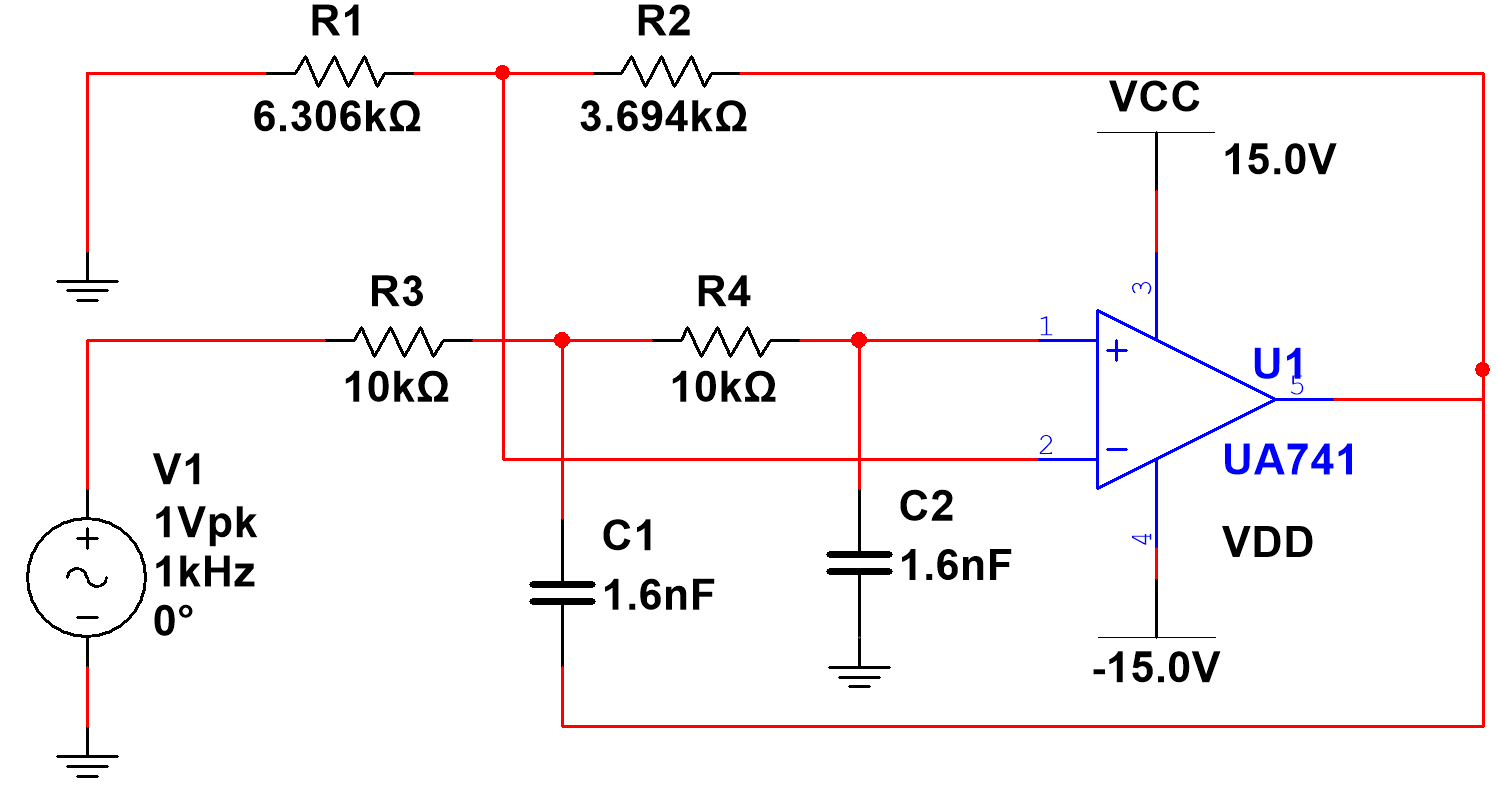
\includegraphics[height=0.2\textwidth]{Images/partAcircuit.png}\\
    \caption{Second Order Butterworth Filter}
    \label{fig:SecondOrderButterworthFilter}
\end{figure}

The calculations to find the resistance $R_1$,$R_2$ and capacitance C, we will be using the formulas from the class notes [1].  
The formulas can also be found from no. 1 in the Appendix. From the formulas, we can see that

\begin{center}
\boxed{R_1 = 6.306k \Omega, R_2 = 3.694k\Omega, C = 1.6nF, A_m = 1.59\frac{V}{V}}
\end{center}
Below is the phase and magnitude plot for our filter:

\begin{figure}[H]
    \centering
    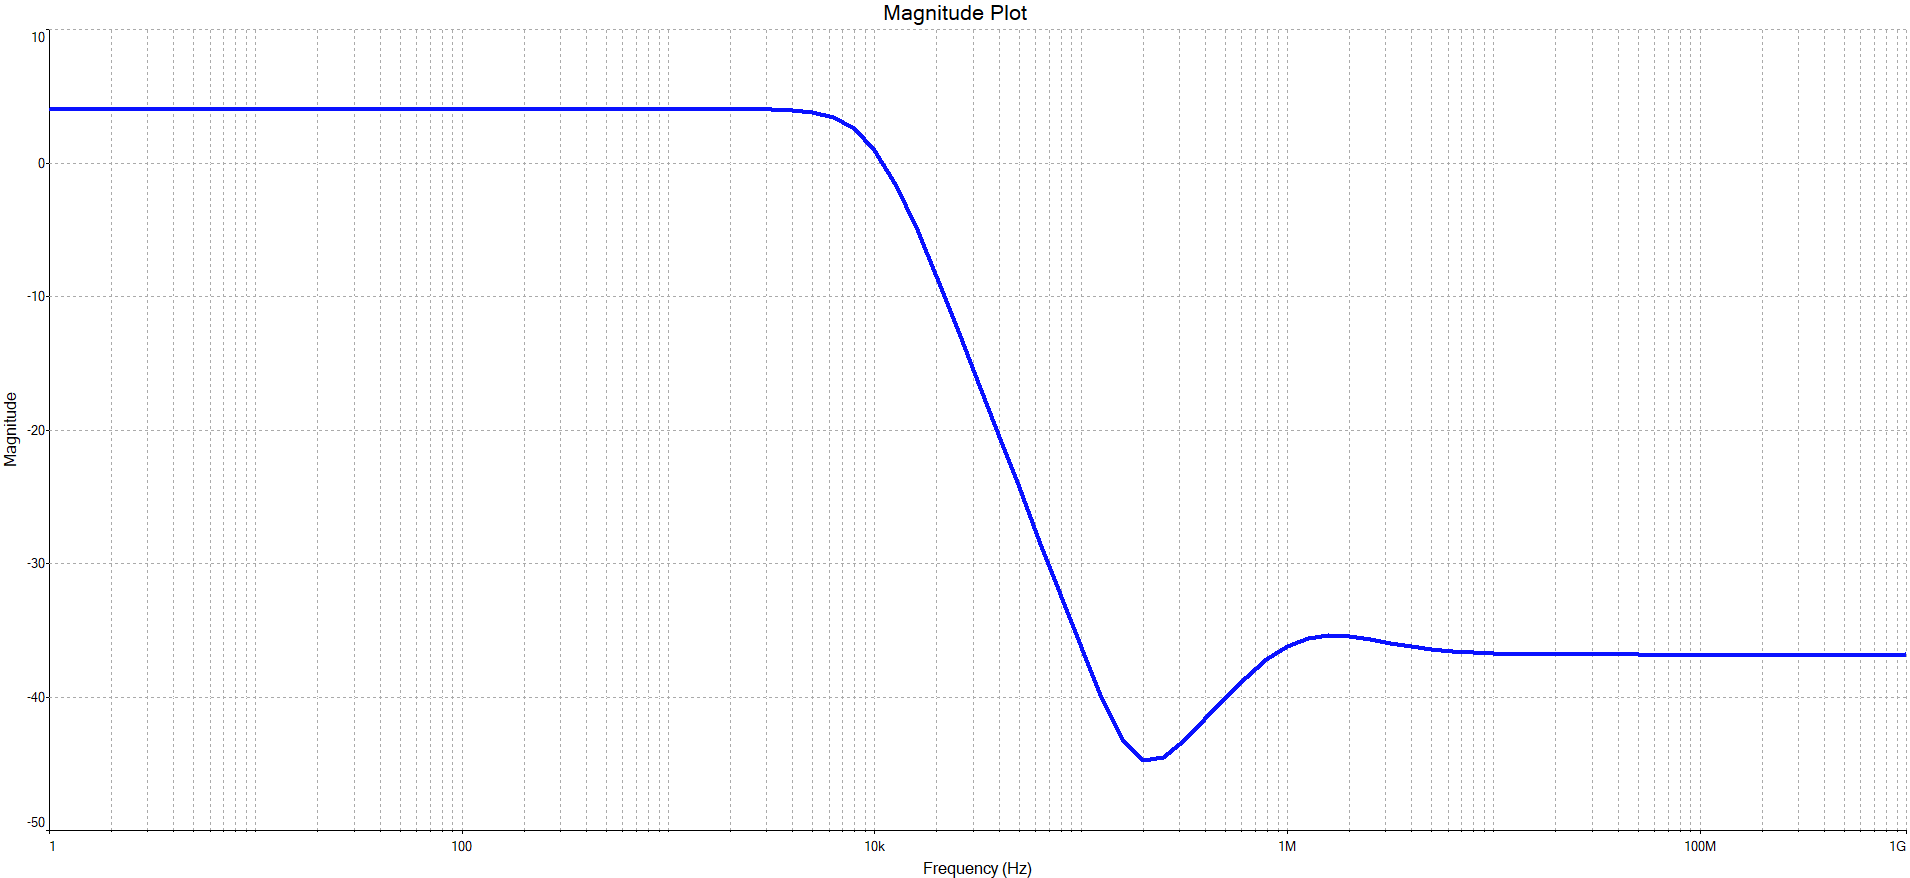
\includegraphics[height=0.45\textwidth]{Images/magnitude_plot.png}\\
    \caption{Bode Magnitude Plot}
    \label{fig:magntitudeplot}
\end{figure}


\begin{figure}[H]
    \centering
    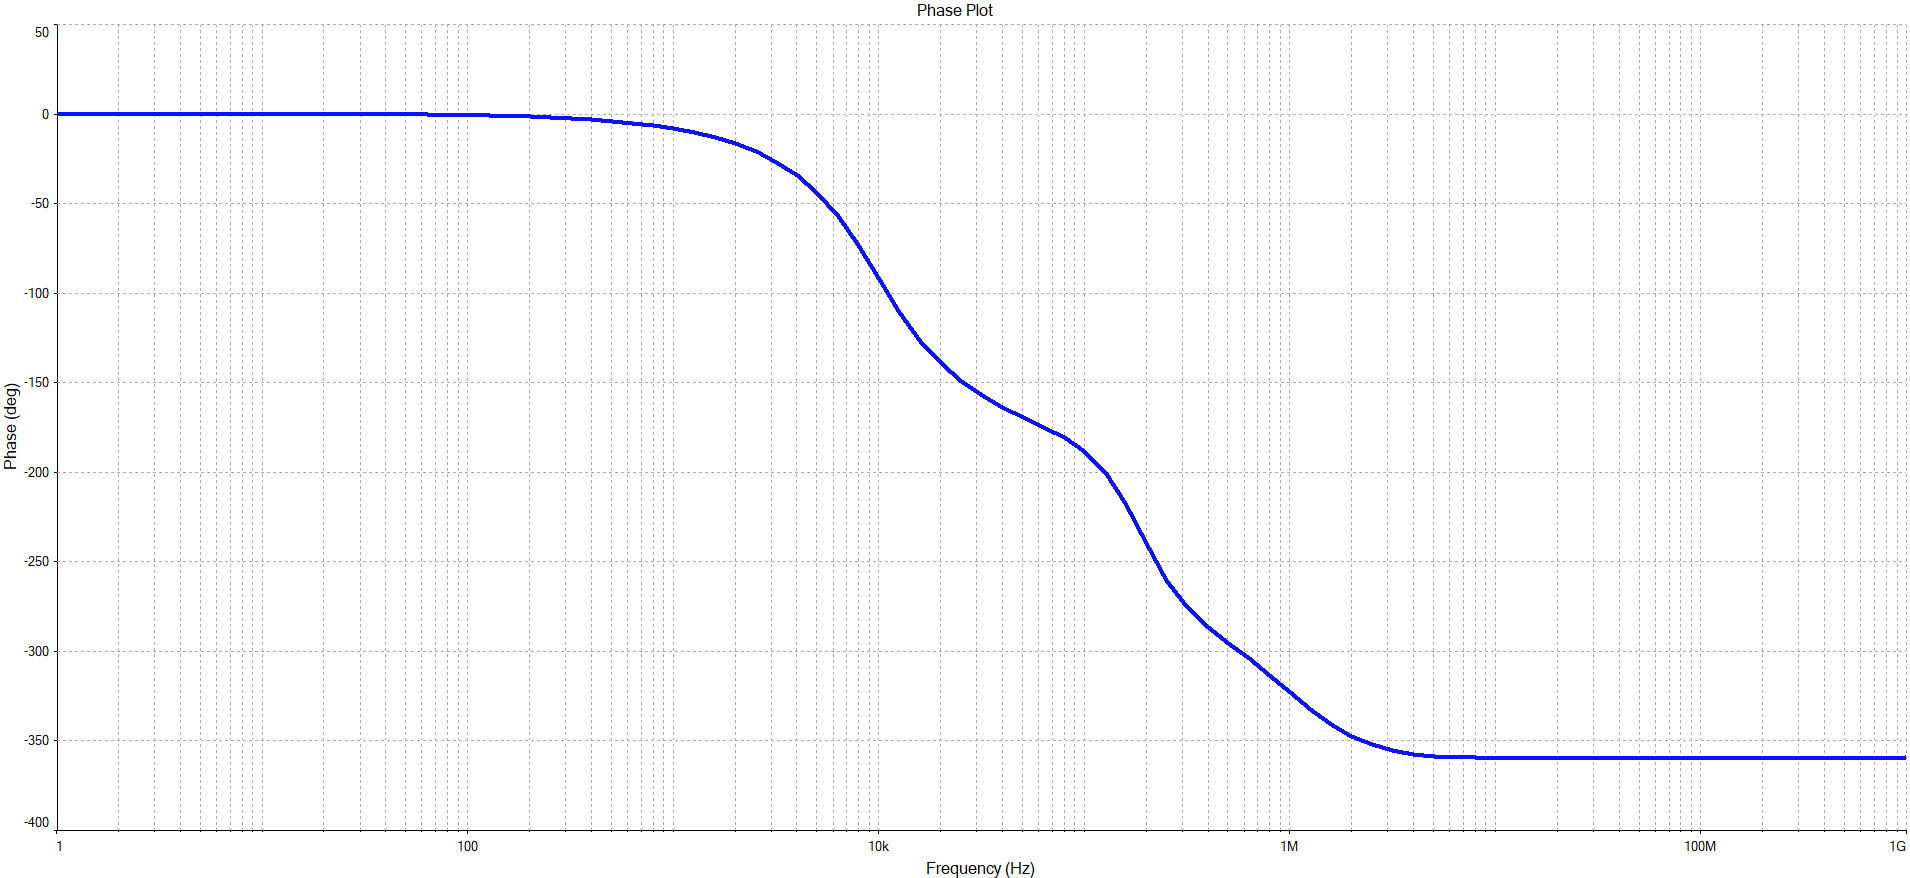
\includegraphics[height=0.45\textwidth]{Images/phase_plot.png}\\
    \caption{Bode Phase Plot}
    \label{fig:phaseplot}
\end{figure}


\subsubsection{Part 2}
For this part, we will be grounding the input, and measuring the output of the OpAmp.
To determine the value of $A_m$ when the circuit begins to oscillate, we need the transfer fucntion. The function is shown below,
where R = $10k\Omega$ and C is the value found previously:
\begin{flalign}
&H(s) = A_M\frac{\frac{1}{(RC)^2}}{s^2+s\frac{3-A_M}{RC}+\frac{1}{(RC)^2}}\nonumber
\end{flalign}
Changing the values of the resistances, we find that the oscillations occour when the resistor values are around$R_1=3k\Omega$ and $R_2 =
7k\Omega$.
The oscillation is shown below:
\begin{figure}[H]
    \centering
    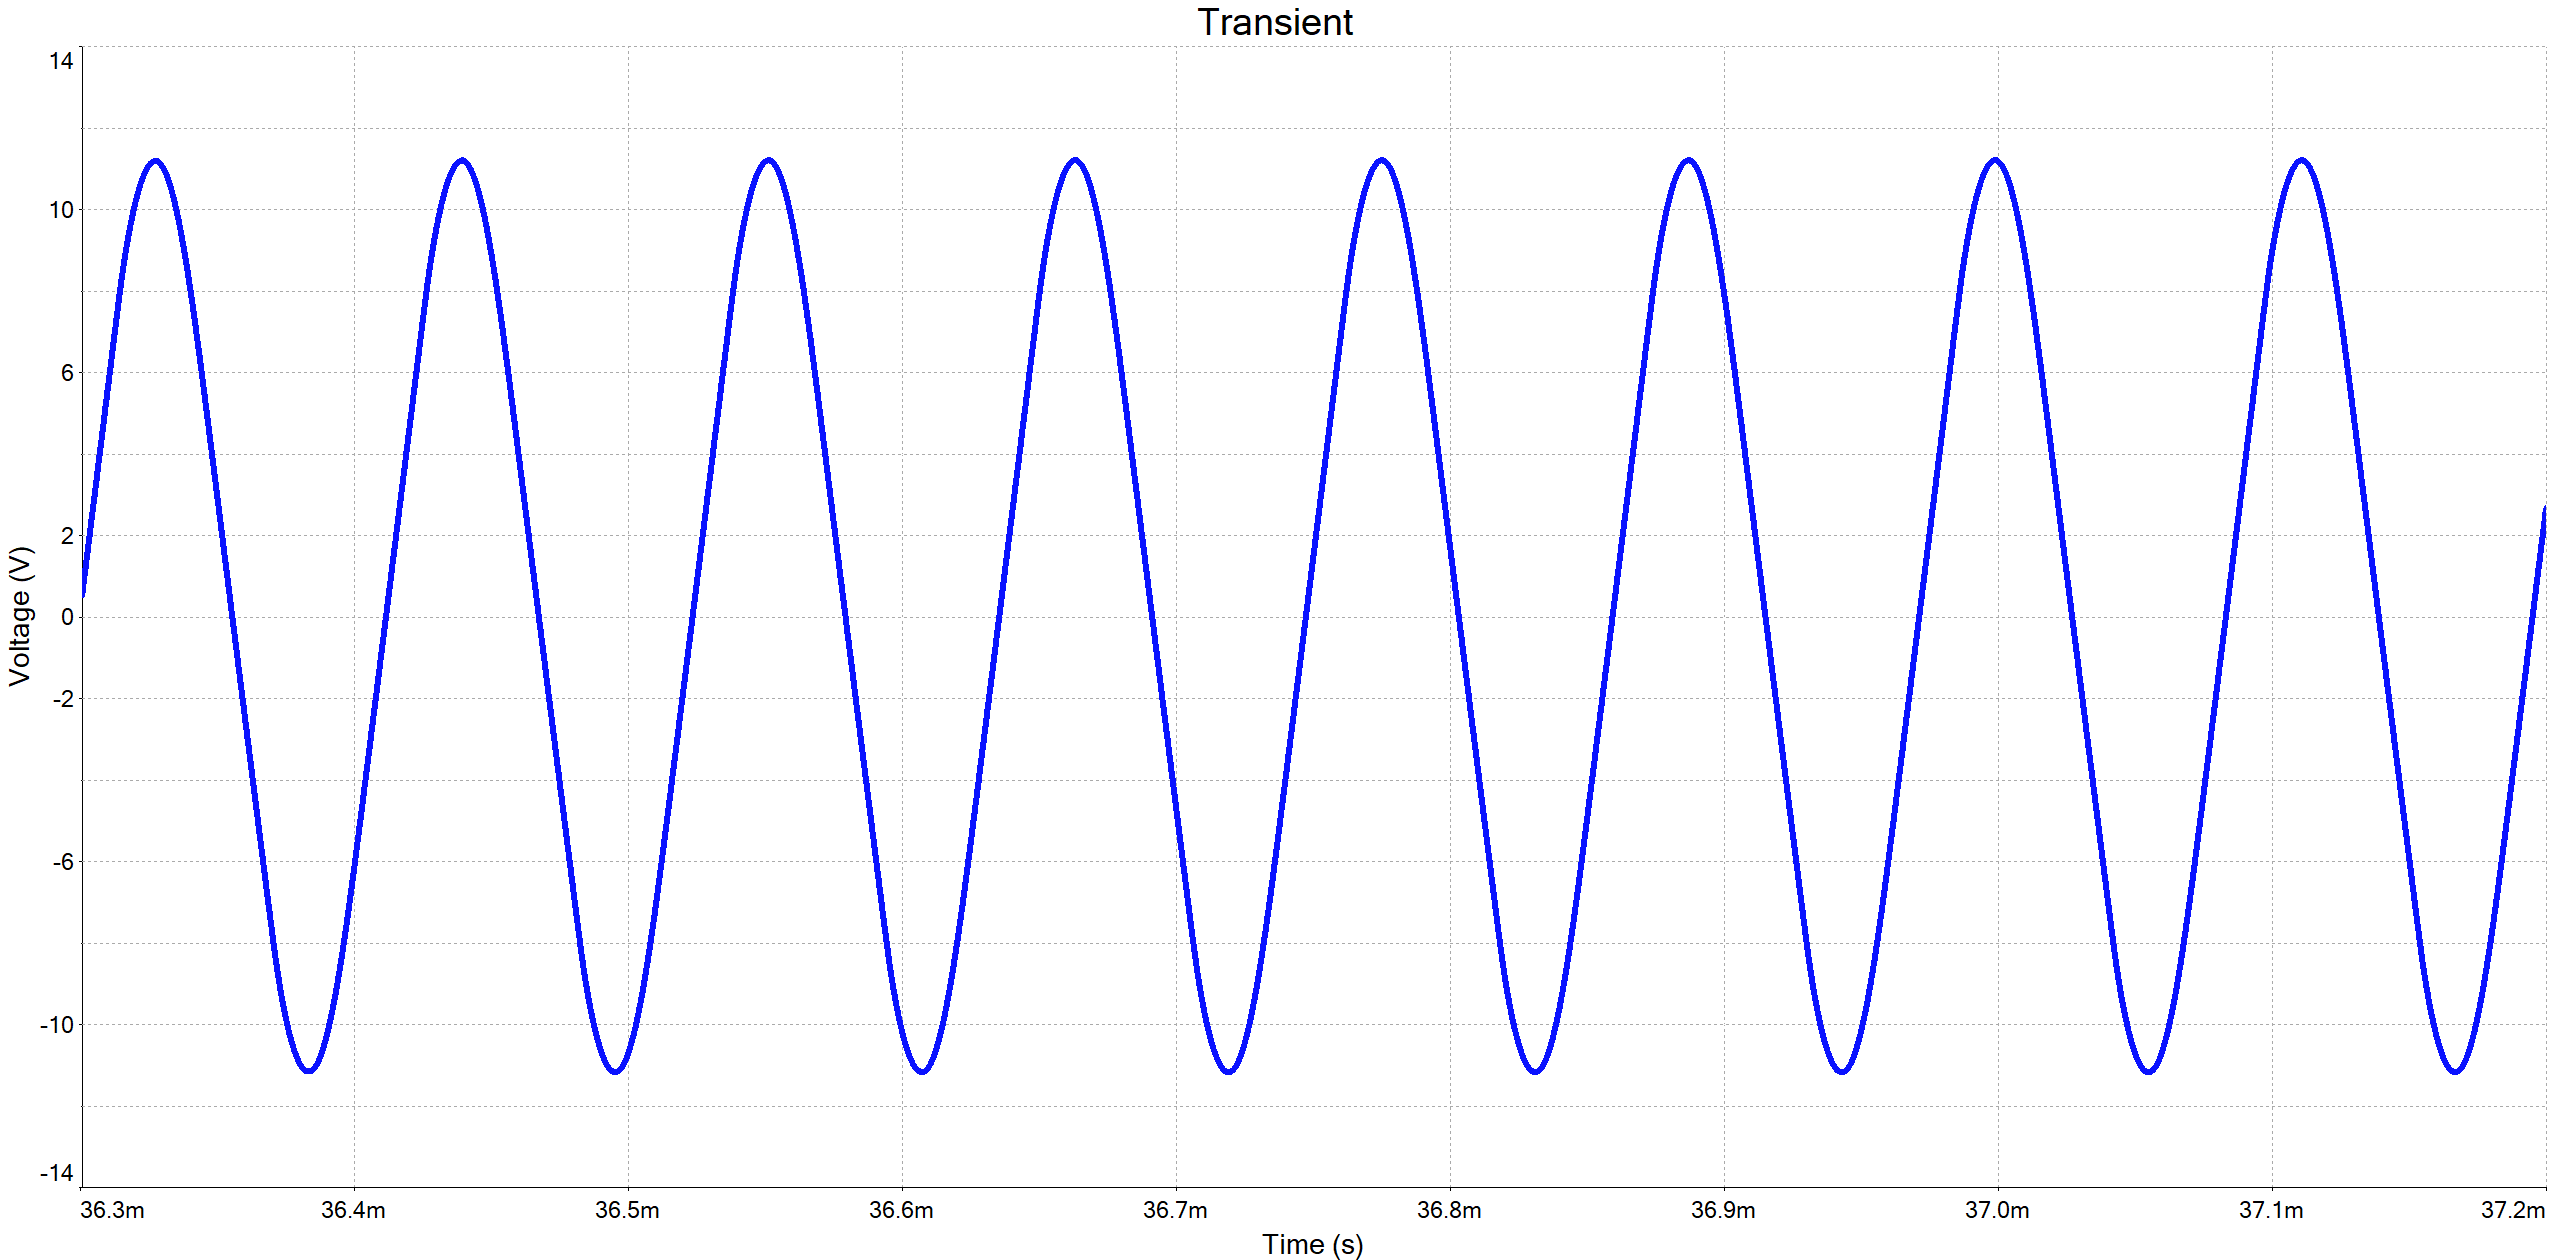
\includegraphics[height=0.45\textwidth]{Images/partatransient.png}\\
    \caption{Oscillating Output}
    \label{fig:oscillatingoutput}
\end{figure}
\FloatBarrier
Using the cursors and measuring the differences between the crests of the plot, we find that the oscillating frequency is 
\boxed{f_o = 8.93kHz}.
Below is the root locus plot:

\begin{figure}
\centering
\begin{minipage}{.5\textwidth}
    \centering
    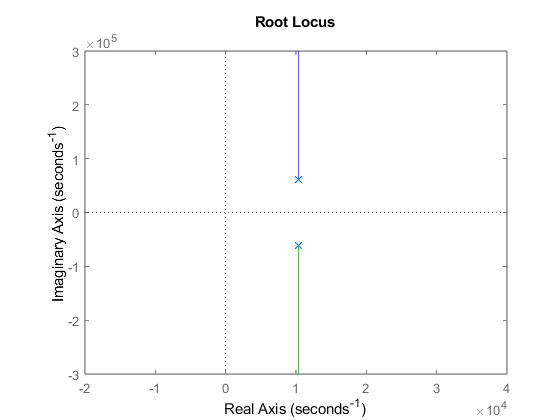
\includegraphics[height=0.7\textwidth]{Images/unstablerootlocus.png}\\
    \caption{Unstable Root Locus Plot}
    \label{fig:unstablerootlocus}
\end{minipage}%
\begin{minipage}{.5\textwidth}
    \centering
    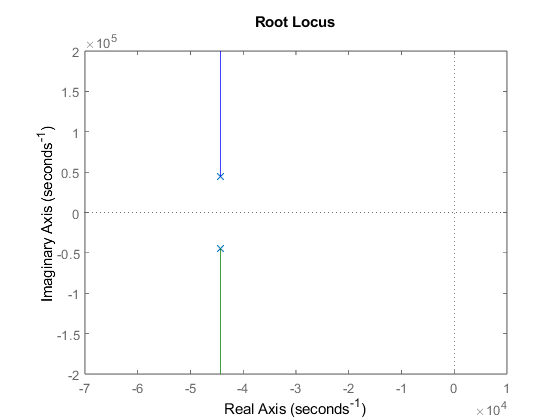
\includegraphics[height=0.7\textwidth]{Images/stablerootlocus.png}\\
    \caption{Stable Root Locus Plot}
    \label{fig:rootlocus}
\end{minipage}
\end{figure}
\FloatBarrier
The root locus plot where $A_M>3$ and $A_M<3$ is Figure \ref{fig:unstablerootlocus} and Figure \ref{fig:rootlocus} respectively. 
We can see from the plot that when the oscillations occour, $A_M$ is greater than 3. This would then cause the system to be 
unstable as shown in Figure \ref{fig:unstablerootlocus}, since the poles are on the right side on the $jw$ axis. When the
poles are on the other side of the $jw$ axis, the system is stable, and doesn't cause the output to oscillate. This happens
when $A_M<3$. The reason why it has to be less than 3 for the system to be stable is because of the characteristic equation in the transfer function. 
If $A_M$ is equal or greater than 3, it causes one of the coefficients in the characteristic equation to be negative, causing instability
in the system and thus, the oscillations occour.

\section{Part B}
Below is our phase shift oscillator circuit:
\begin{figure}[H]
    \centering
    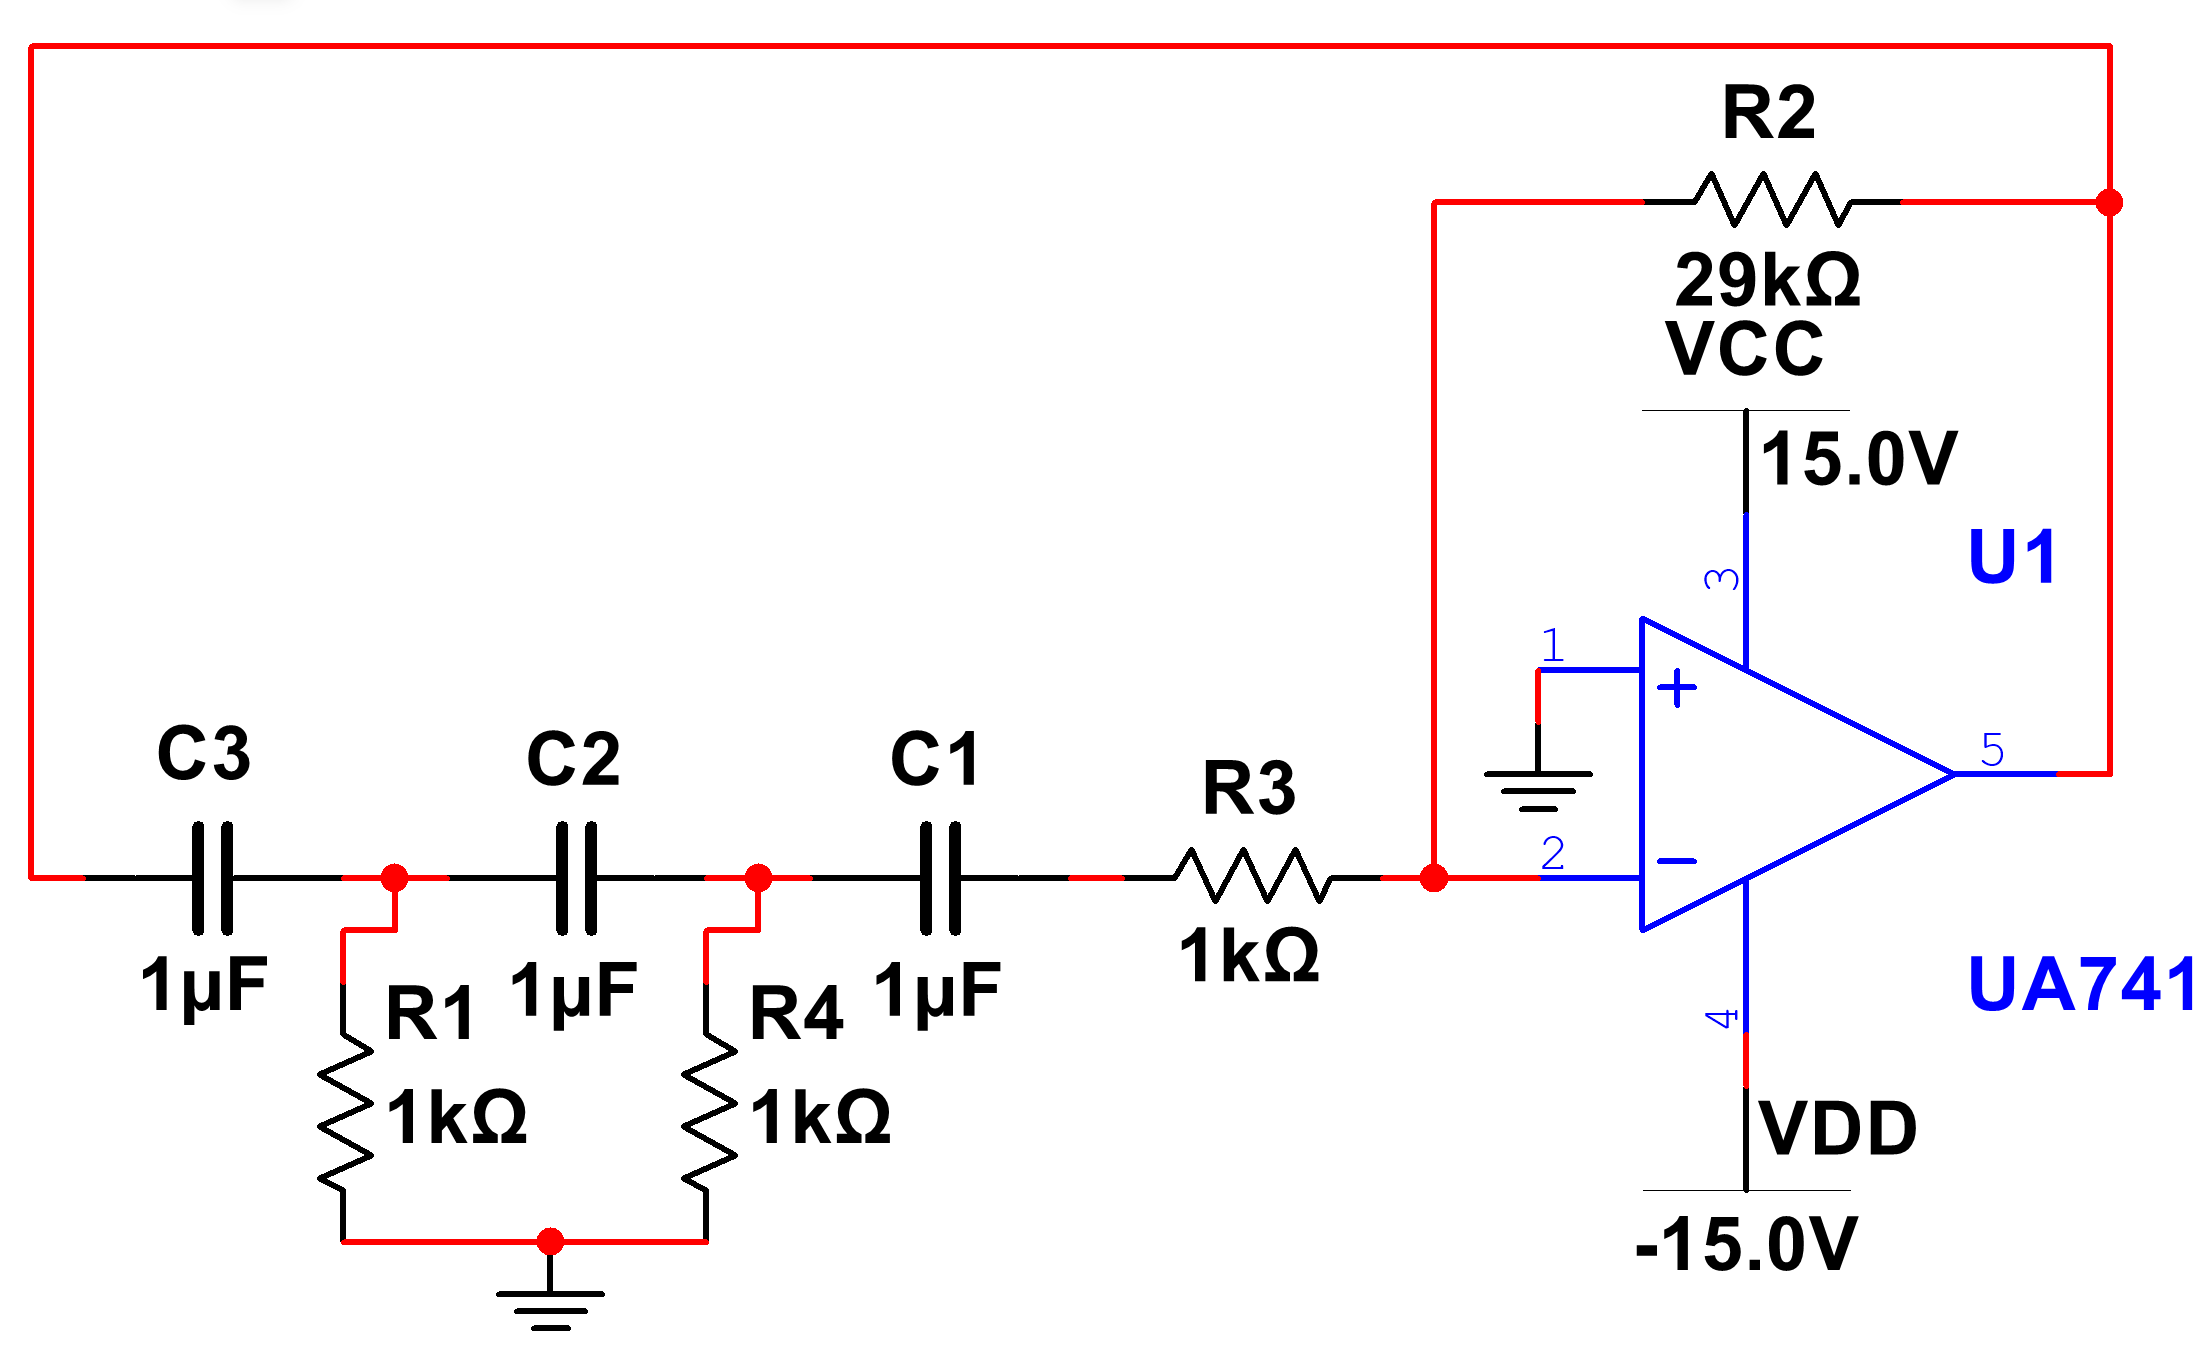
\includegraphics[height=0.3\textwidth]{Images/phaseoscillatorcircuit.png}\\
    \caption{Phase Shift Oscillator Circuit}
    \label{fig:oscillatorcircuit}
\end{figure}
\FloatBarrier

To find the proper value of the 29R resistor, we will simulate the output response for a very large amount of time (in this case, 1000 seconds
was used). Simulating with just $29k\Omega$ we find that the output amplitude eventually decays to zero. Increasing the resistor
to $29.1k\Omega$ makes the output amplitude to be sustained indefinitely. 

Plotting the output of the circuit with the values given in the project document [2] and the increased 29R resistor , we find that 
the output oscillates as shown: 

\begin{figure}[H]
    \centering
    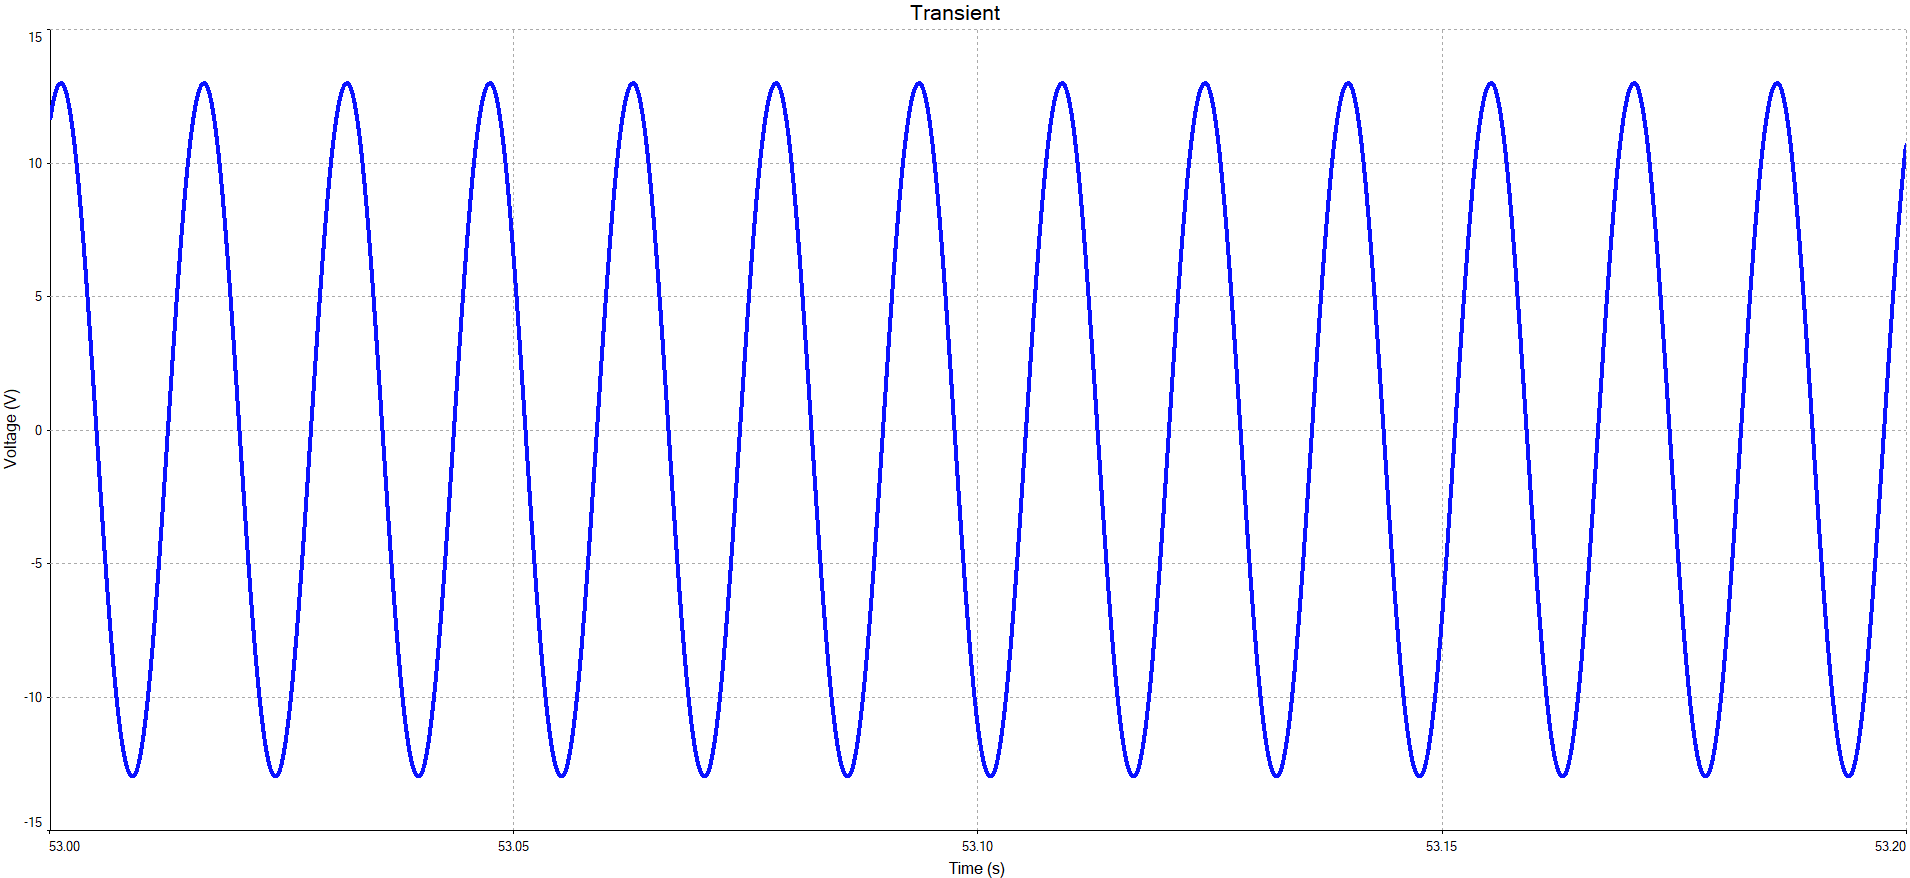
\includegraphics[height=0.45\textwidth]{Images/partbtransient1x.png}\\
    \caption{Circuit Output With Unchanged Circuit Elements}
    \label{fig:oscillatorcircuit1x}
\end{figure}

\begin{figure}[H]
    \centering
    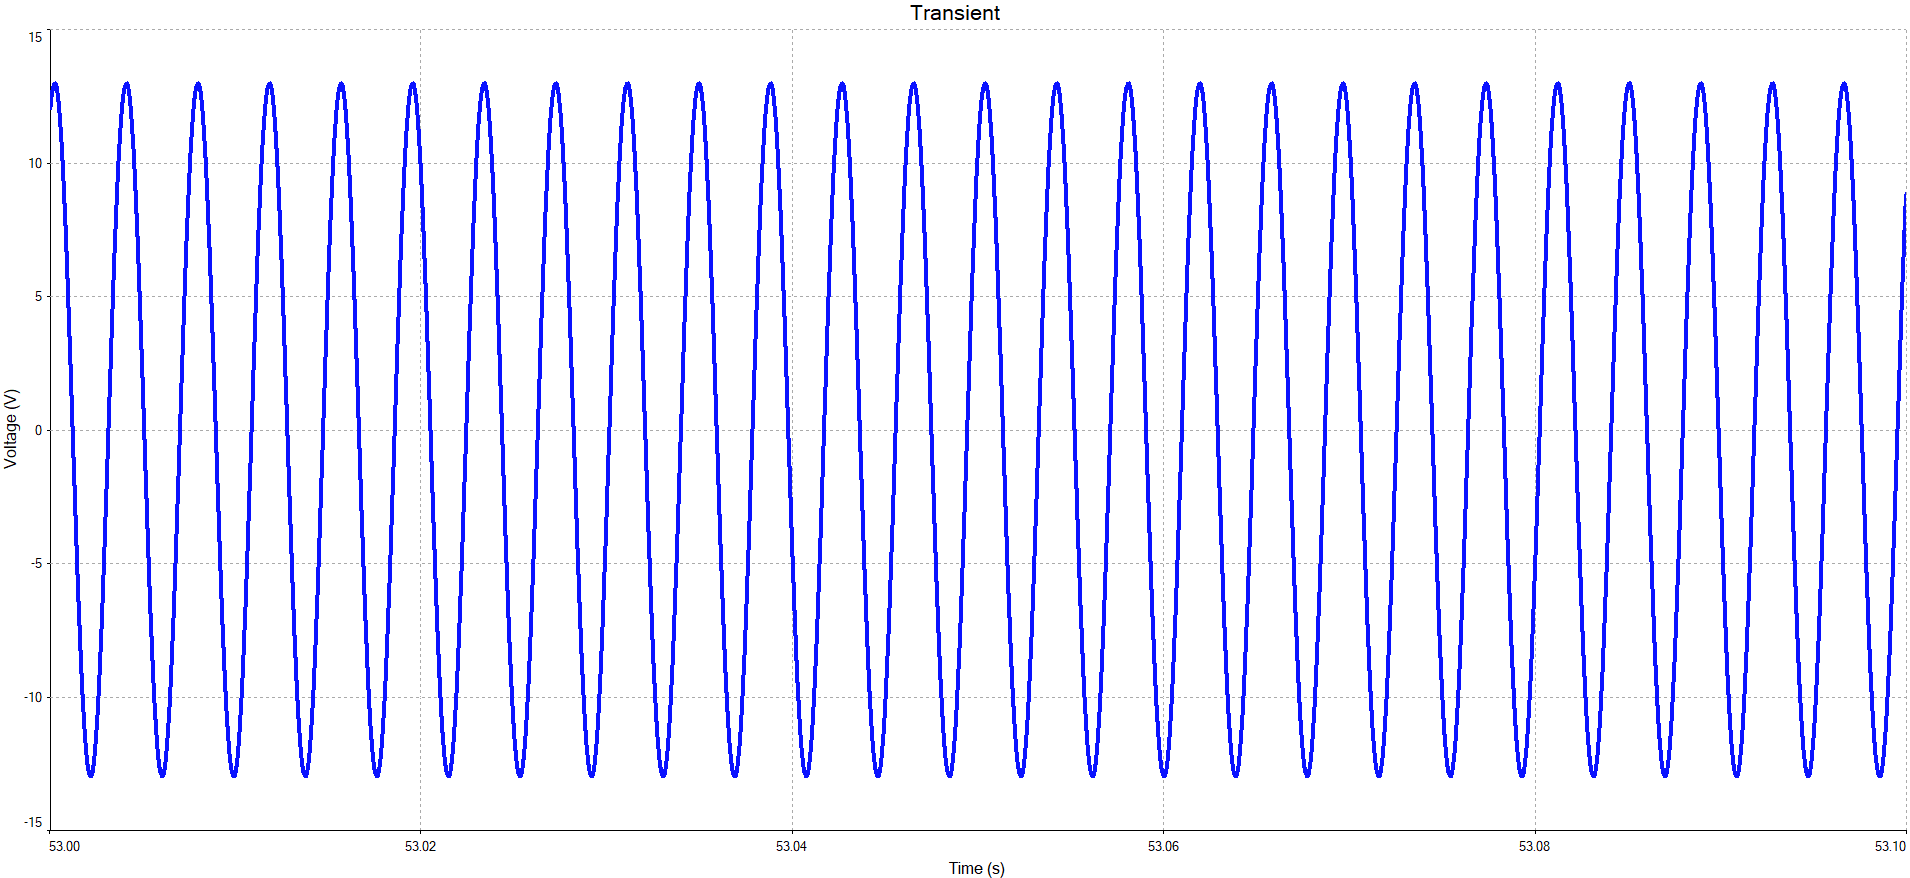
\includegraphics[height=0.45\textwidth]{Images/partbtransient0.5x.png}\\
    \caption{Circuit Output With Half Circuit Elements}
    \label{fig:oscillatorcircuit0.5x}
\end{figure}

\begin{figure}[H]
    \centering
    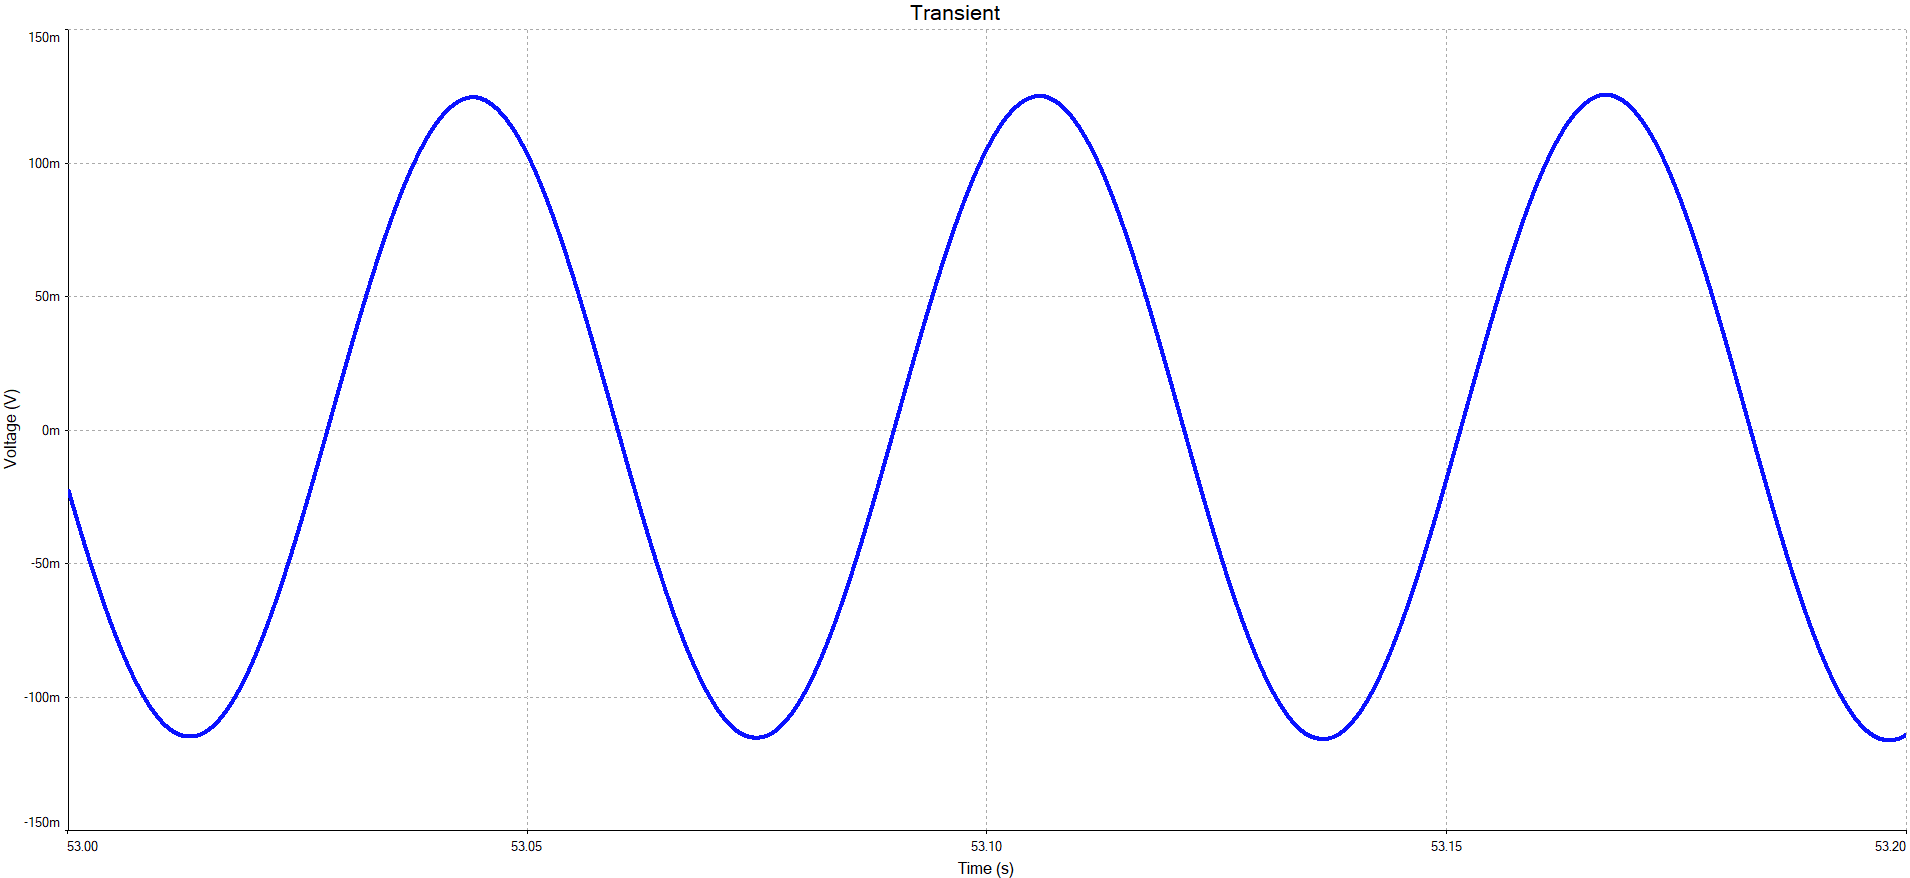
\includegraphics[height=0.45\textwidth]{Images/partbtransient2x.png}\\
    \caption{Circuit Output With Double Circuit Elements}
    \label{fig:oscillatorcircuit2x}
\end{figure}
From class notes[1], we can calculate the output frequency with:
\begin{flalign}
    &f=\frac{1}{2\pi RC \sqrt{6}} \nonumber
\end{flalign} 
In the table below, the multiplier indicatates the circuit element value (ex. 0.5x indicates $R=500\Omega$ and C = $0.5\mu$ F).
Comparing the calculated and measured frequencies for each modified circuit:

\begin{table}[h!]
    \centering
    \resizebox{0.5\textwidth}{!}{%
    \begin{tabular}{l|l|l|l}
    
    R and C Multiplier& 0.5x & 1x & 2x \\ \cline{1-4}
    Calculated $f_o(Hz)$ & 259.899 & 64.975 & 16.244 \\ \cline{1-4}
    Measured $f_o(Hz)$ & 259.067 & 64.872 & 16.221 \\ \cline{1-4}
    \% Error & 0.32 & 0.15 & 0.14
    \end{tabular}%
    }
    \caption{Calculated and Measured Frequencies}
    \label{CalculatedMeasuredFrequencies}
\end{table}
\FloatBarrier

We can observe that the calculated and measured values are very close to each other. The way that a phase shift oscillator
works is that a third order RC circuit is connected behind an amplifier with a negative gain[5]. In this case, the negative feedback
is supplied by the 29R resistor, with our OPAMP as our amplifier. The reasoning behind the increase of the 29R resistor, is that our negative gain
has to be larger than the gain of the input circuit[5]. The gain of the input in this case was represented by the 29R resistor.
We observed that with just 29R, the output was not sustained, and eventaully decayed to zero. Once the resistor was increased,
we observed that the output was stable. 

\section{Part C}
Below is our Feedback Circuit:
\begin{figure}[H]
    \centering
    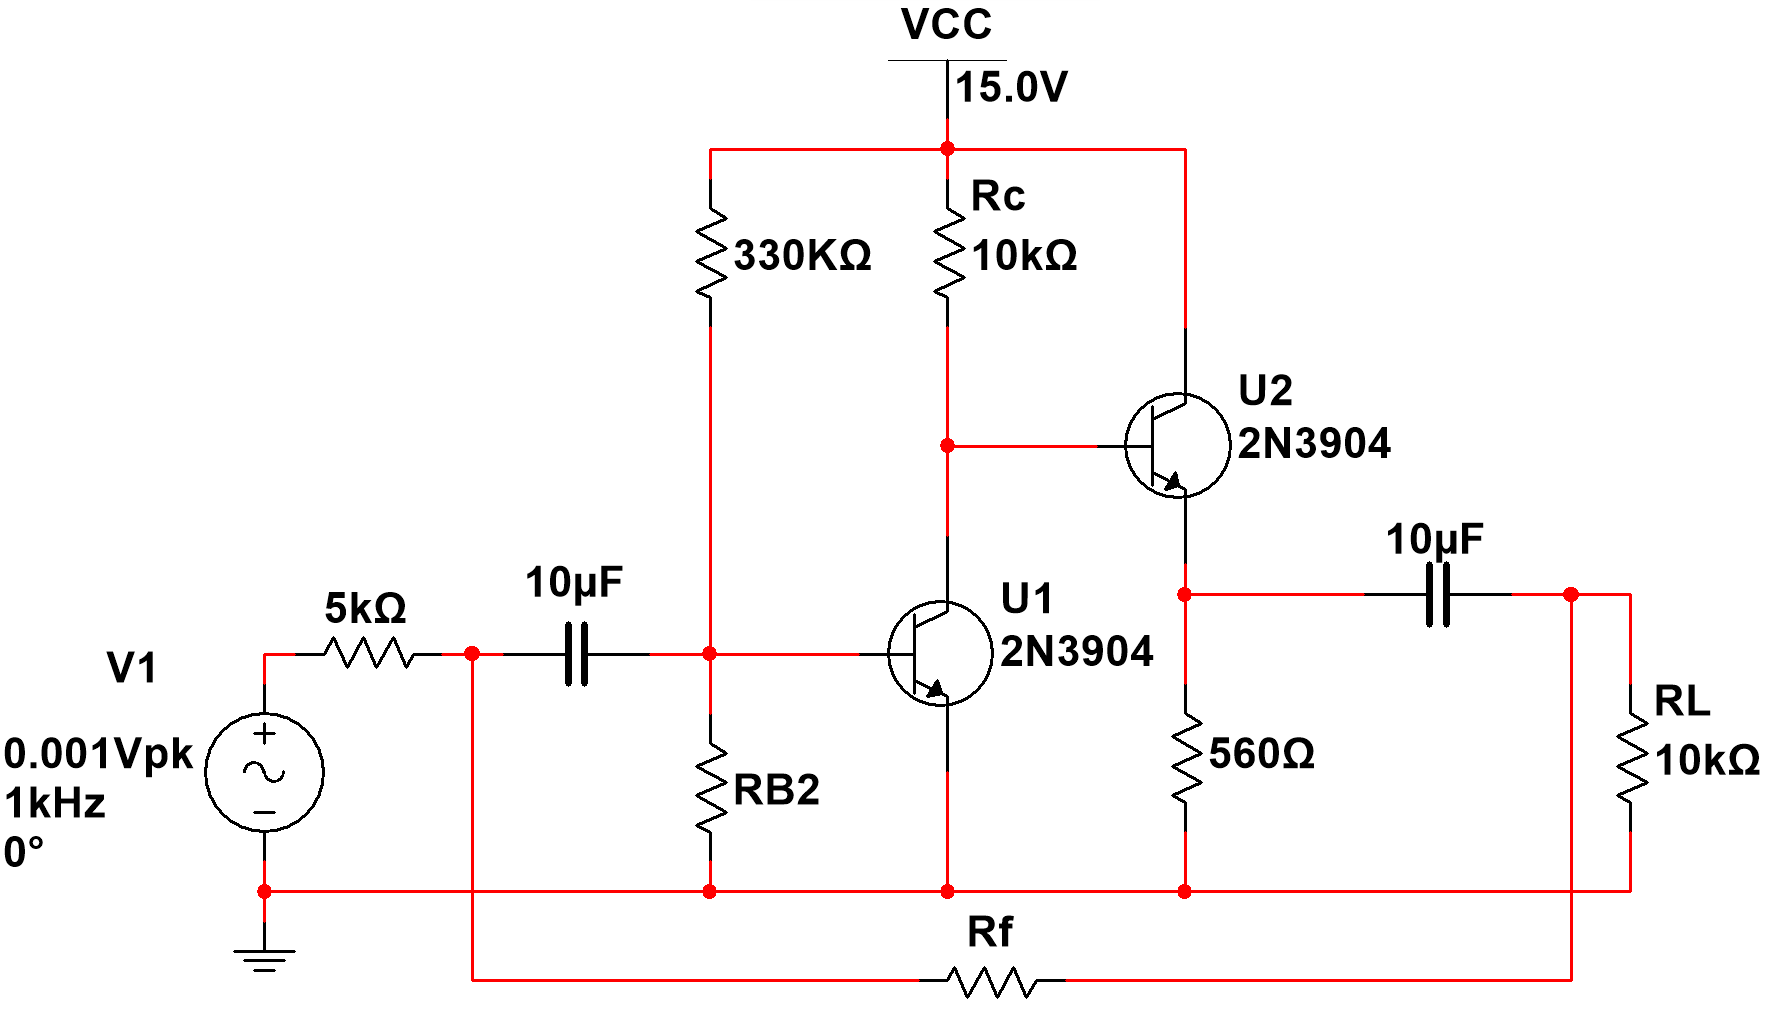
\includegraphics[height=0.35\textwidth]{Images/partCcircuit.png}\\
    \caption{Feedback Circuit}
    \label{fig:feedbackcircuit}
\end{figure}

Since we want to find the value of $R_{B2}$ that creates the largest open-loop gain at 1kHz, we will be setting our
input voltage at 1kHz at 1mV. To find the value, we will be doing a parameter sweep with a transient response to 
find which resistance value results in the largest gain. We find that after doing the parameter sweep,
the value $R_{B2}$ to be around \boxed{20k\Omega}. Resistance values above $20k\Omega$
, we find that the output amplitude decreases. The parameter sweep is shown below:

\begin{figure}[h!]
    \centering
    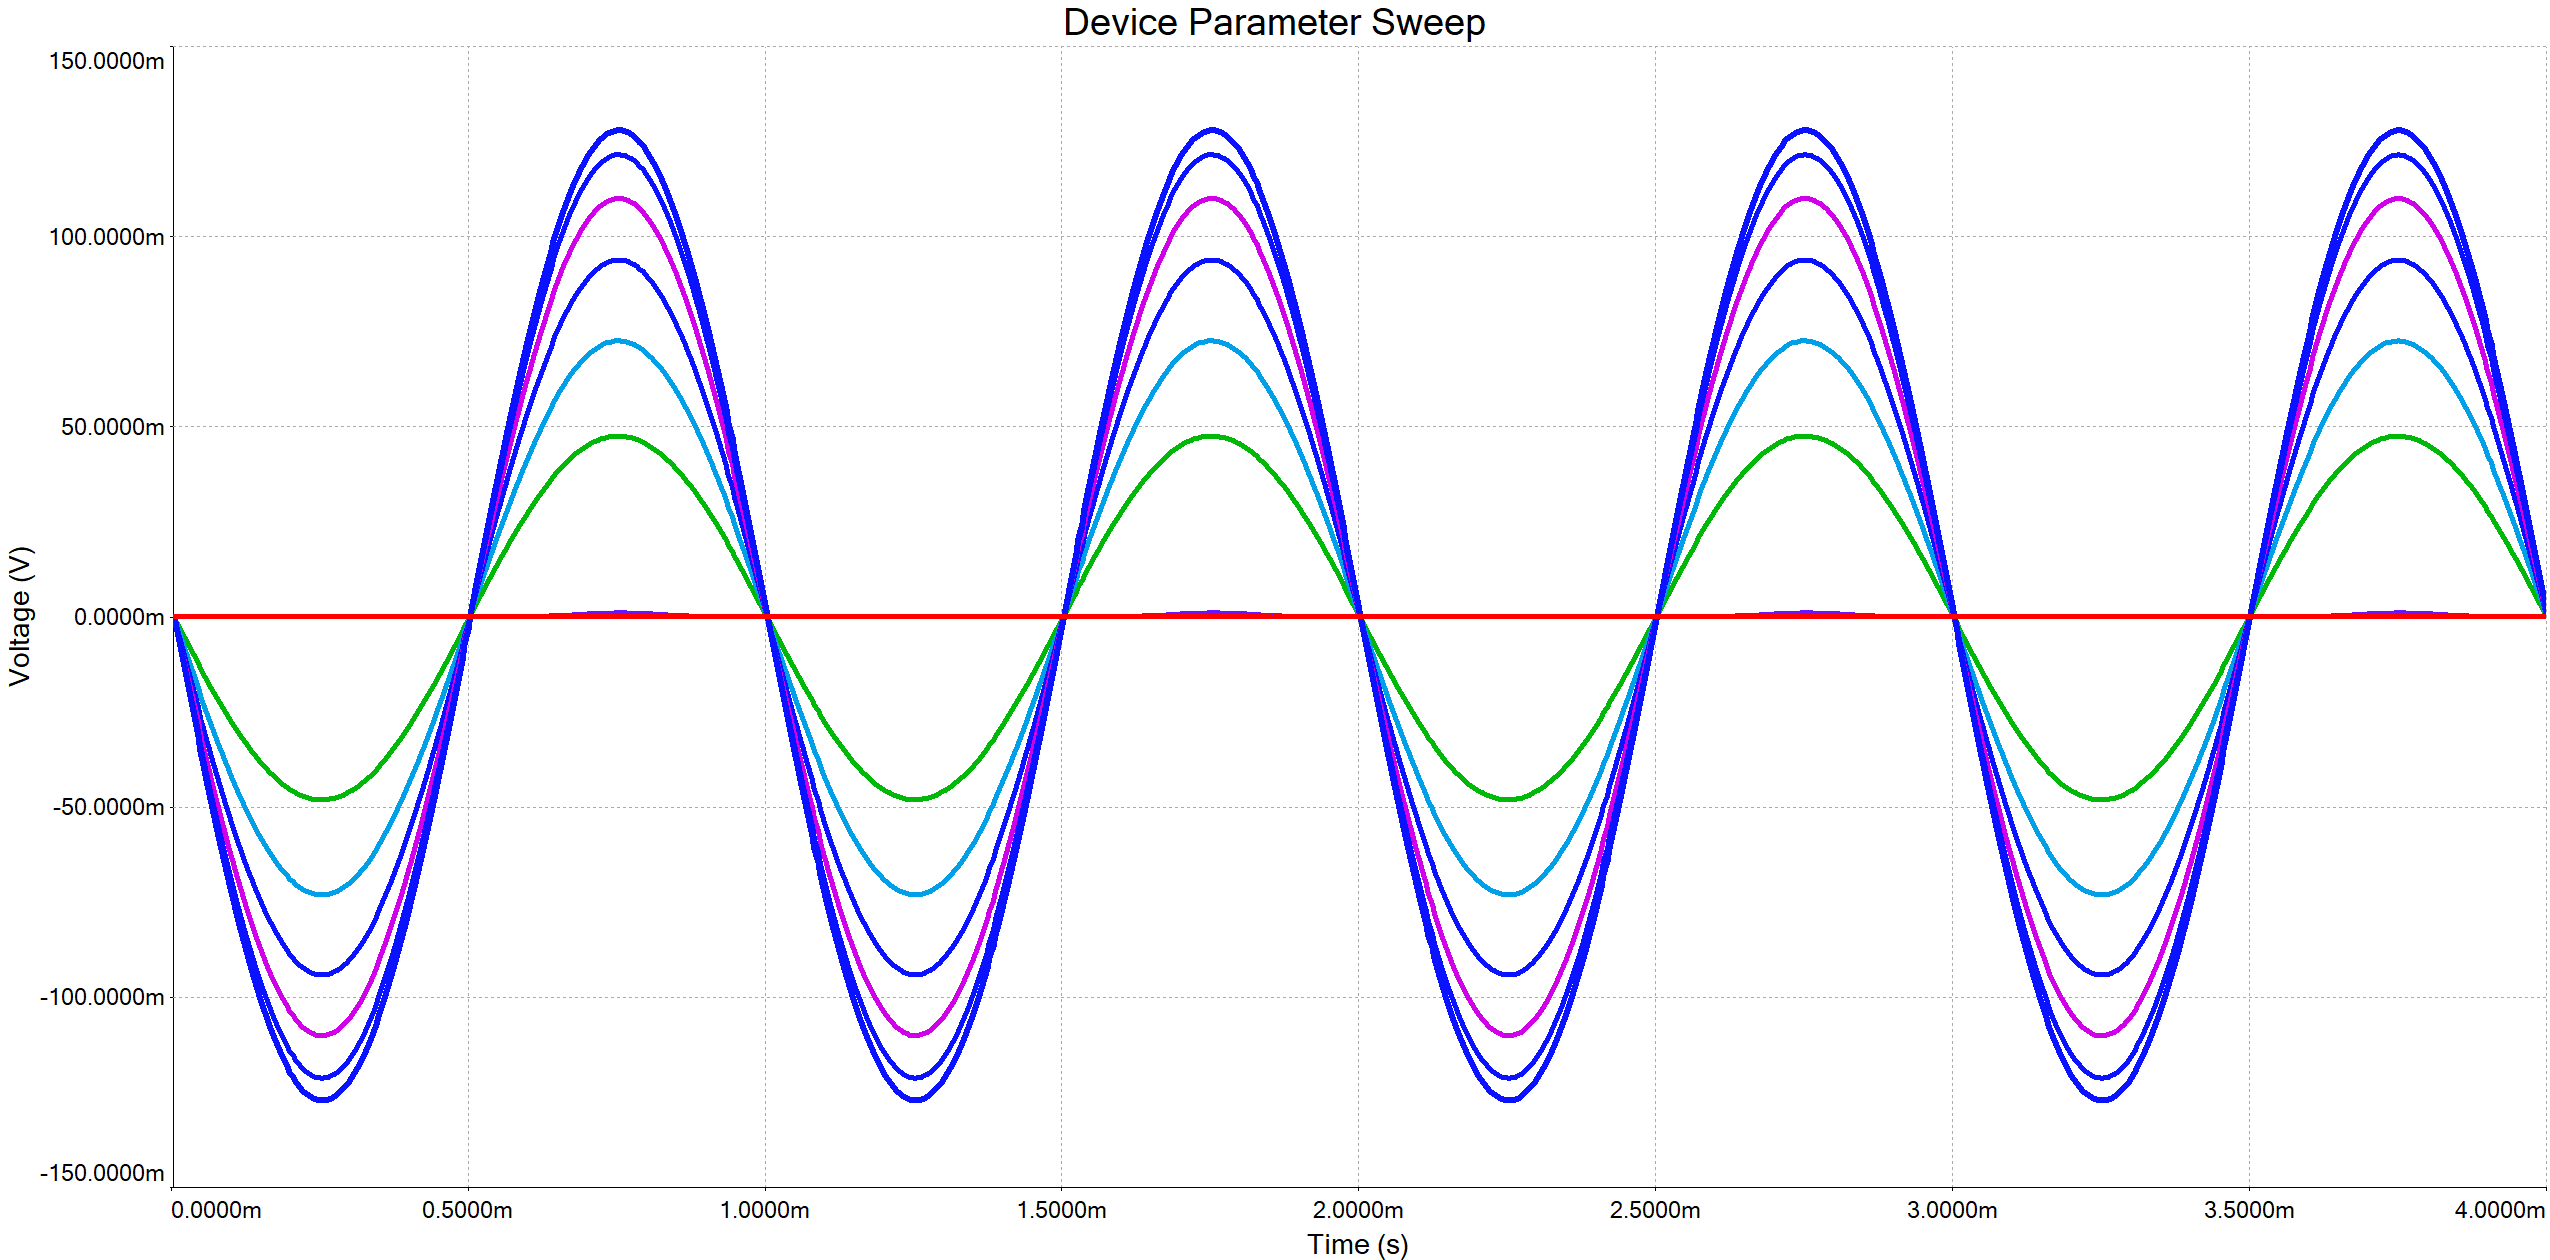
\includegraphics[height=0.45\textwidth]{Images/parametersweep.png}\\
    \caption{Parameter Sweep with $R_{B2}$ and Transient Response}
    \label{fig:parametersweep}
\end{figure}
\FloatBarrier

\subsection{Part 1}
To measure the DC Operating points, we will be using the DC Circuit below:
\begin{figure}[h!]
    \centering
    \includegraphics[height=0.3\textwidth]{Images/partCDC.png}\\
    \caption{Feedback DC Circuit}
    \label{fig:feedbacdccircuit}
\end{figure}
\FloatBarrier
For this project, we will be assuming that $V_T$= 0.025V. We can use these formulas to 
calculate our transistor parameters:
\begin{center}
    $r_\pi= \frac{V_T}{I_B}$ ,$\beta = \frac{I_C}{I_B}$ and $g_m = \frac{\beta}{r_\pi}$
\end{center}
Here are the DC Operating points, with our measured $r_\pi,g_m$, and $h_{FE}$:
\FloatBarrier
\begin{table}[h!]
    \centering
    \begin{tabular}{l|lllllllll}
     & $I_C$ & $I_B$ & $I_E$ & $V_C$ & $V_B$ & $V_E$ & $g_m$ & $r_\pi$ & $h_{FE}$ \\ \cline{1-10}
    Q1 & 1.29mA & 10.8uA & 1.31mA & 1.90V & 0.654V & 0V & 0.05 & 2.315k$\Omega$ & 119  \\ \cline{1-10}
    Q2 & 2.19mA & 15.4uA & 2.21mA & 15V & 1.90V & 1.23V & 0.09 & 1.623k$\Omega$ & 142
    \end{tabular}%
    \caption{DC Operating Points}
    \label{DC Operating Points}
\end{table}

\subsection{Part 2}
\subsubsection{Finding Measured Open Loop Frequency Responce and I/O Impedance}
Here is the open loop frequency response plot:
\begin{figure}[h!]
    \centering
    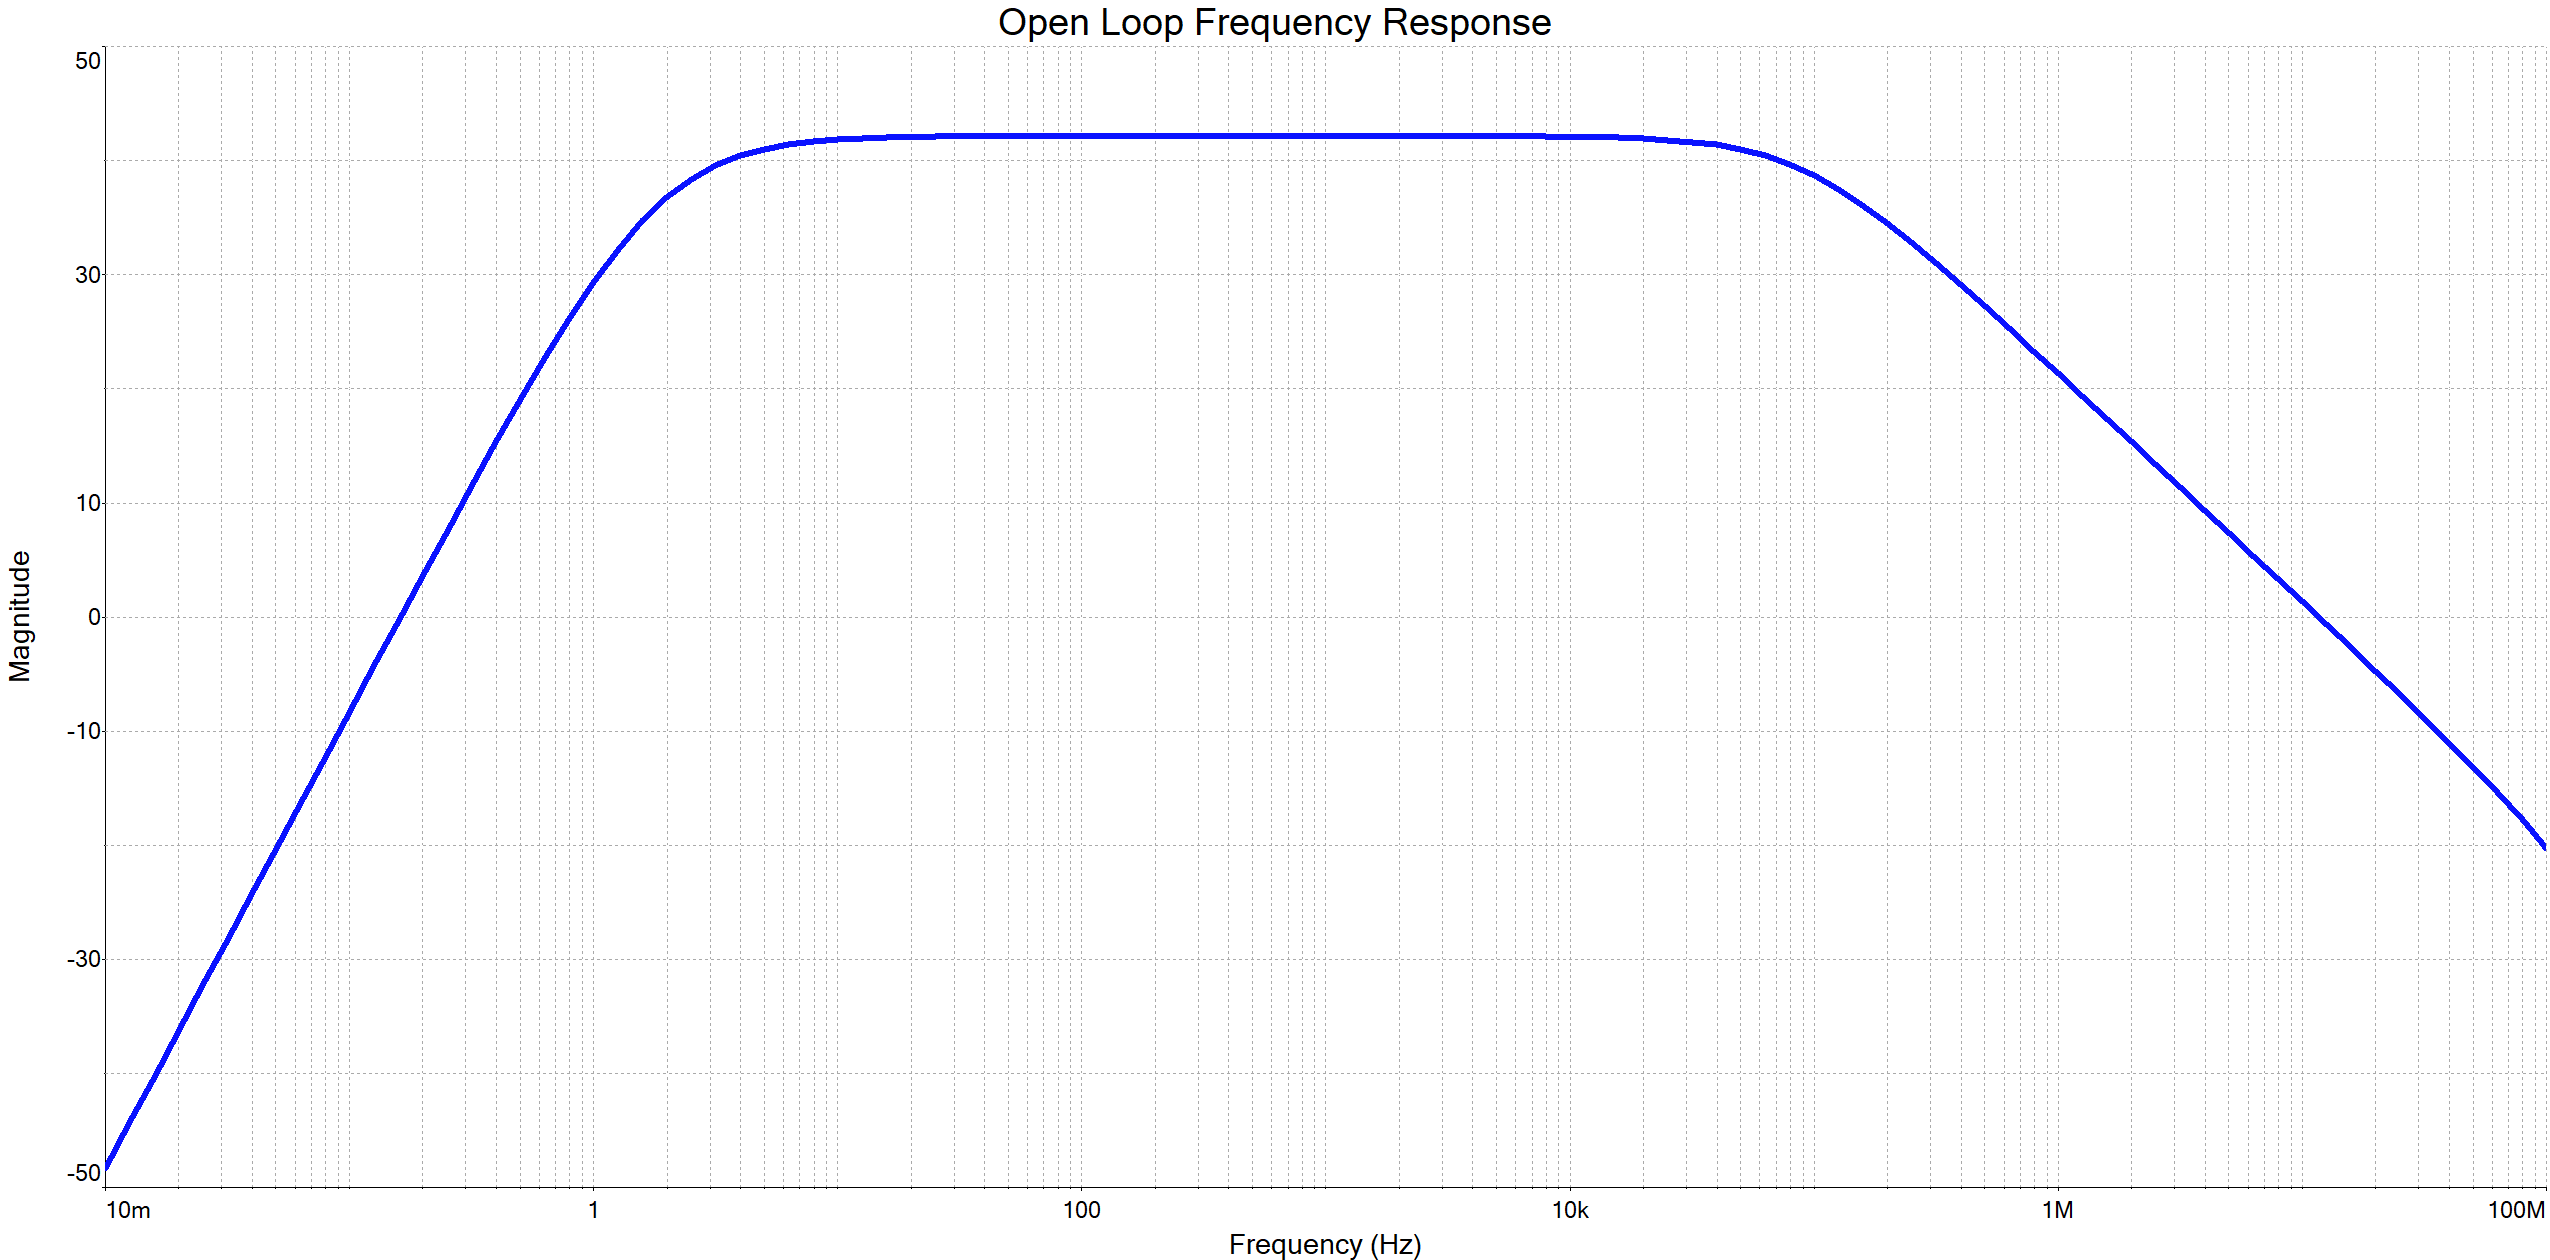
\includegraphics[height=0.45\textwidth]{Images/partCbode.png}\\
    \caption{Open Loop Frequency Response}
    \label{fig:olfreqresponse}
\end{figure}
\FloatBarrier
Measuring with the cursors in our simulation software, we find that the 
3dB points are: 
\begin{center}
    \boxed{w_{L3dB} = 2.9219 *2\pi [\frac{rad}{s}], w_{H3dB} = 91.3083*2\pi*10^3[\frac{rad}{s}] } 
\end{center}
We can also find our mid-band gain \boxed{A_m = -127.557\frac{V}{V}} from the frequency 
response plot.
In order to find the input and output resistance at 1kHz, we will be measuring the voltage 
and current at the input, and we will be adding a test source at the output and grounding the
input for the output impedance measurements. After measuring, we find: 
\begin{center}
$R_{in} = \frac{240\mu V}{93.4nA}$ = \boxed{2.569k\Omega}, 
$R_{out} = \frac{707\mu V}{11.4 \mu A} = $ \boxed{62.017\Omega}
\end{center}

\subsubsection{Predicted Closed Loop Frequency Response}
For this section, we will need to calculate our circuit parameters and input and 
output resistance at 1kHz with $R_f=100k\Omega$. To do this, we need to know our circuit's 
topology. Since the output is sampled by $R_f$ and mixes the current from the output into the
input, we can determine that our feedback circuit uses shunt-shunt topology. Due to this,
we will be using y-parameters to perform our calculations. Below is the y-parameter matrix
we will be using:
\begin{center}
$\begin{bmatrix}
        I_1 \\
        I_2
\end{bmatrix}$ =
$\begin{bmatrix}
    V_{1} \\
    V_{2}  
\end{bmatrix}$ 
$\begin{bmatrix}
    y_{11} && y_{12} \\
    y_{21} && y_{22} 
\end{bmatrix}$
\end{center}
To find the value of $y_{11}$, we set $V_2=0$. Then, we find that \boxed{y_{11}=\frac{1}{R_f}}
for our $y_{12}$ parameter, we set $V_1=0$. We also know that $\beta=y_{12}$. It is found as
\boxed{y_{12}=\beta=\frac{-1}{R_f}}.For $y{21}$, we find that it's effect is small compared
relative to the other gain values, so we will not consider it in calculations. For $y_{22}$, we 
set $V_1=0$ and find that \boxed{y_{22} = \frac{1}{R_f}}.
\subsubsection{Gain Calculations}
Since our circuit is in shunt-shunt topology, our open-loop will be  $\frac{V_{out}}
{I_{in}}$. Therefore, we need to convert our input to the amplifier from a voltage source 
to a current source. To do this, we will be transforming our source from a voltage source 
in series with our source resistance to a current source in parallel to our source resistance. 
Doing this, our resulting input current is \boxed{I_{in} = \frac{V_s}{5k\Omega}}. So we find
our open loop gain to be:
\begin{flalign}
    &A^{'}= \frac{V_{out}}{I_{in}} = \frac{V_{out}}{\frac{V_s}{5k\Omega}}  = \frac{V_{out}}
    {V_{s}}(5k\Omega) = -127.557\frac{V}{V}*(5k\Omega) = \boxed{-637.786k\frac{V}{A}} \nonumber
\end{flalign}

Now, we are able to find our gain with feedback. The formula used
can be found in the class notes[1]. It is found as:
\begin{flalign}
&A_f = \frac{A^{'}}{1+\beta A^{'}} = -86.446k\frac{V}{A} \nonumber
\end{flalign}
Since the units we need is $\frac{V}{V}$ we convert our input to a voltage source,
and this can be done by dividing $A_f$ by $5k\Omega$. After doing this, we find
\boxed{A = -17.289 \frac{V}{V}}. Which is our closed loop gain.

\subsubsection{3dB Calculations}
To calculate the $w_{3dBf}$ (3dB frequencies with feedback), we can use the 
following formulas from the class notes[1]. The frequencies are found to be:
\begin{flalign}
&w_{Hf3dB} = (w_{H3dB})(1+A^{'}\beta) = (91.308k*2\pi)(1+\frac{-1}{100k\Omega}*-637.786k\frac{V}{A}) = \boxed{ 4233.189k \frac{rad}{s}}\nonumber\\
&w_{Lf3dB} = \frac{w_{L3dB}}{1+A^{'}\beta} = \frac{2.9219 *2\pi}{1+\frac{-1}{100k\Omega}(-637.786k\frac{V}{A})} =\boxed{2.488 \frac{rad}{s}} \nonumber
\end{flalign}

\subsubsection{Input and Output Resistance Calculations}
To calculate our input and output resitance values with feedback, we can 
use our open loop resistance values and formulas[1] to calculate the values
we eventually find:
\begin{flalign}
&R_{if} =  \frac{R_{in}}{1+A^{'}\beta} = \frac{2.569k\Omega}{1+\frac{-1}{100k\Omega}(-637.786k\frac{V}{A})} =\boxed {348.204\Omega}\nonumber \\
&R_{of} = \frac{R_{out}}{1+A^{'}\beta} = \frac{62.017\Omega}{1+\frac{-1}{100k\Omega}(-637.786k\frac{V}{A})} =  
\boxed{8.406\Omega}\nonumber
\end{flalign}

Here is our closed loop frequency response curve:

\begin{figure}[h!]
    \centering
    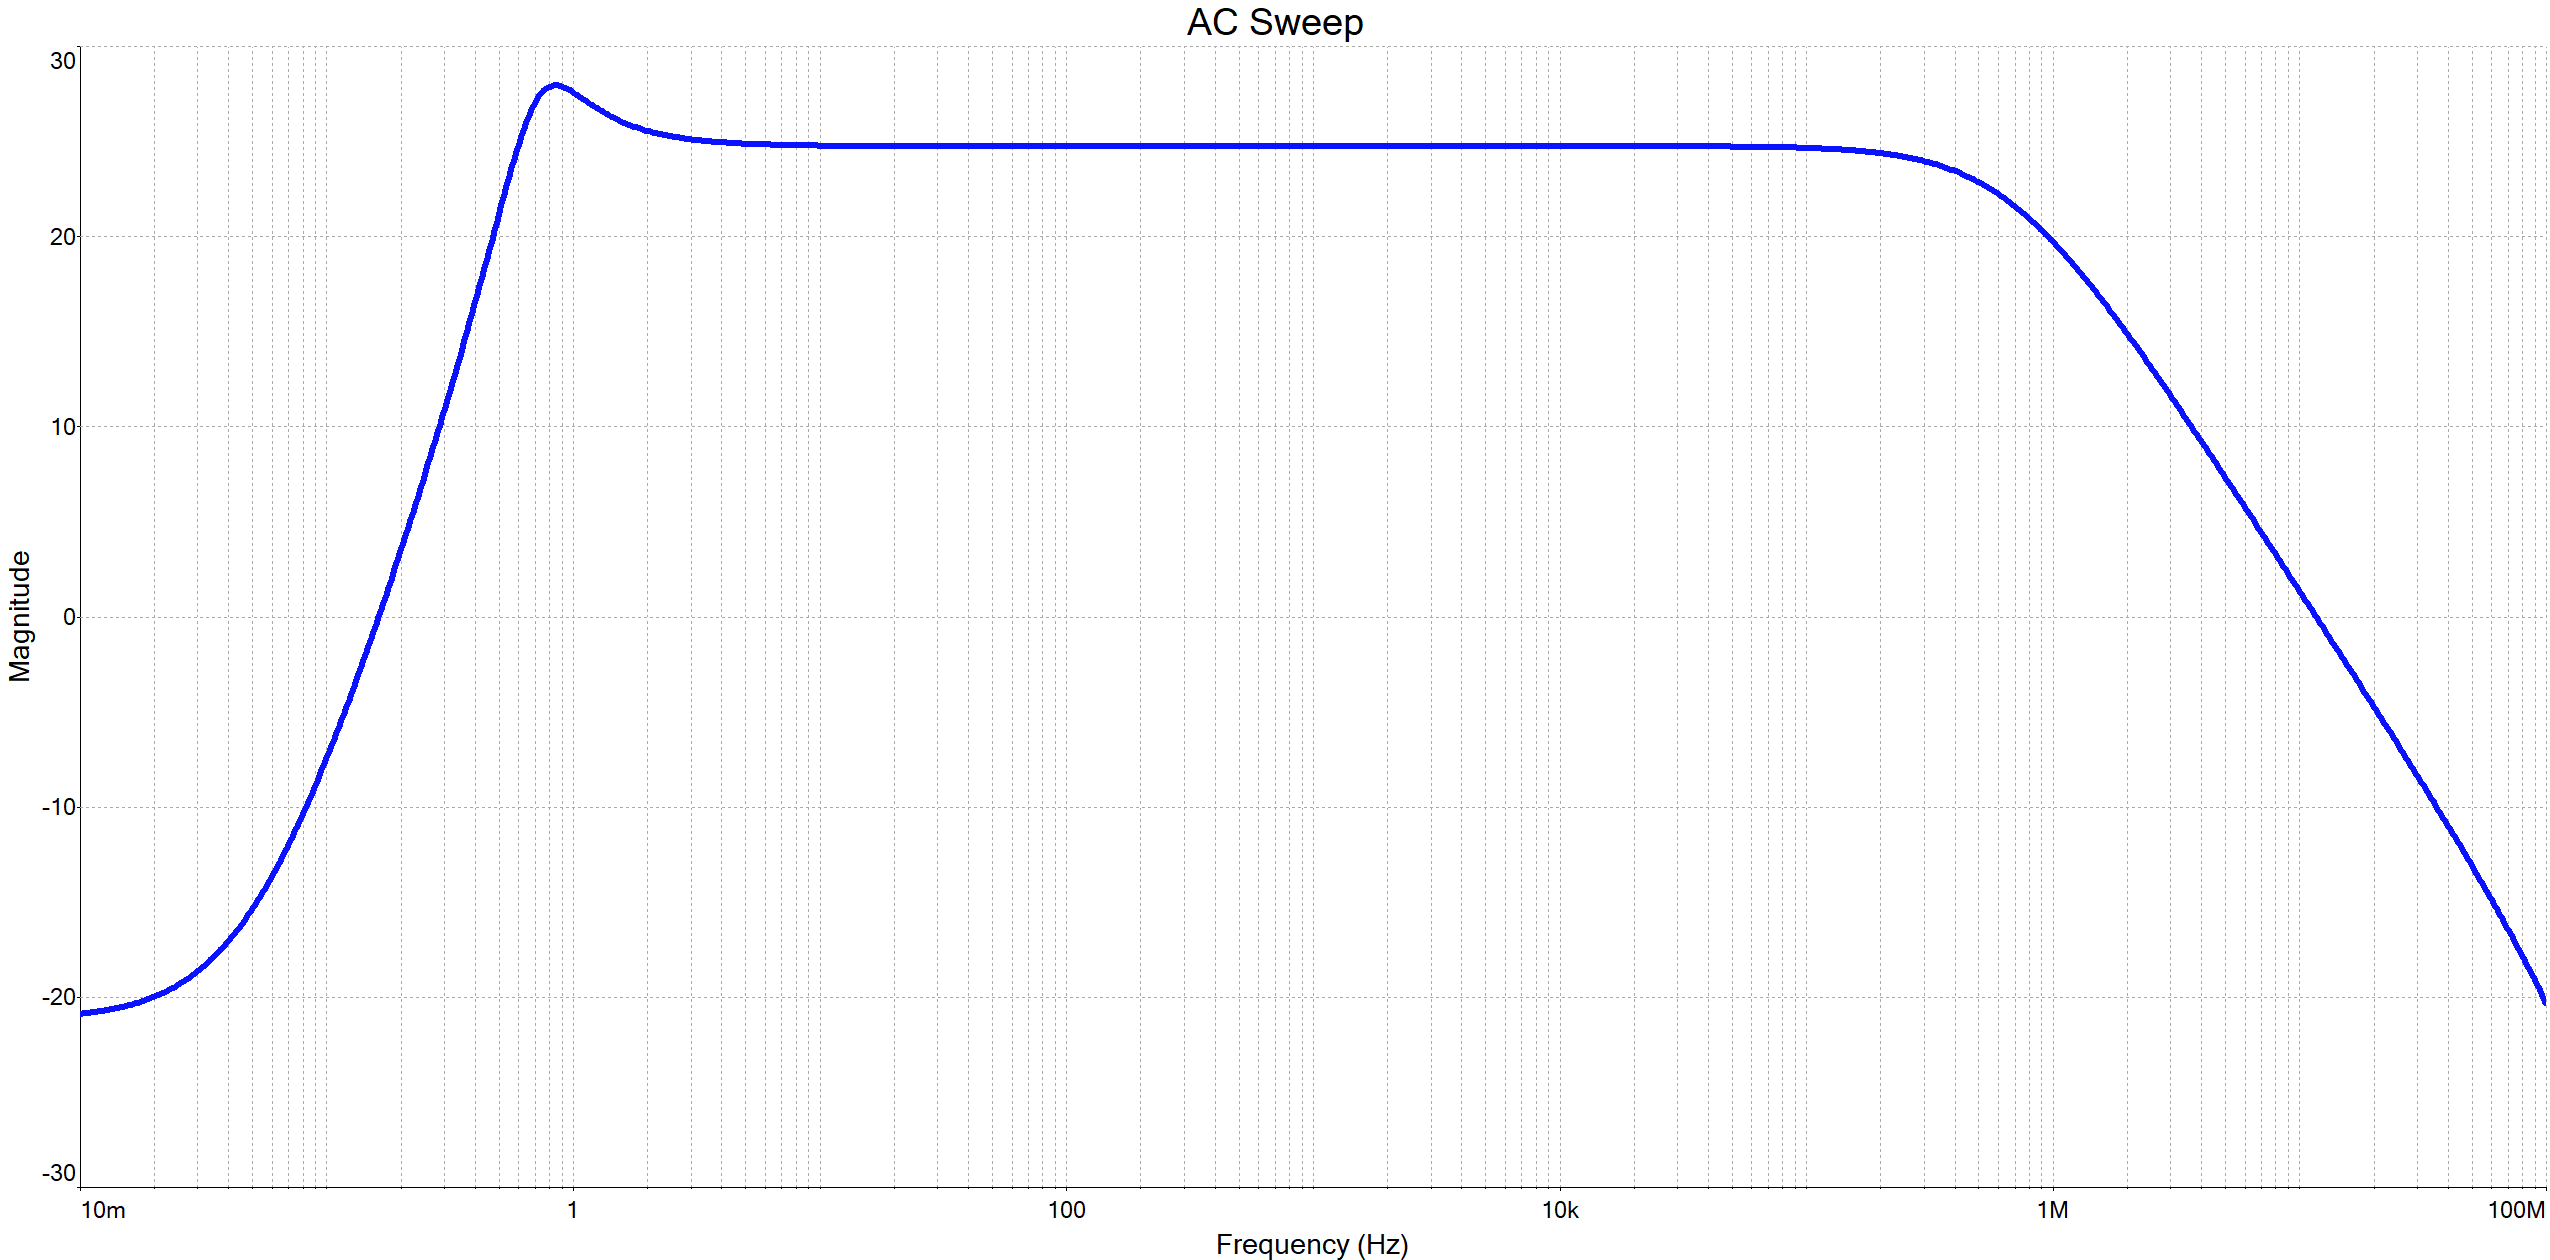
\includegraphics[height=0.45\textwidth]{Images/partcfeedbackbode.png}\\
    \caption{Closed Loop Frequency Response}
    \label{fig:clfreqresponse}
\end{figure}
\FloatBarrier
From this, we can measure the following values:

\begin{table}[h!]
    \centering
    \begin{tabular}{l|lllll}
        
     & $w_{L3dB}$ & $w_{H3dB}$ & $R_{in}$ & $R_{out}$ & $A_f$ \\ \cline{1-6}
    Measured & 3.221[$\frac{rad}{s}$] & 4257.361k[$\frac{rad}{s}$] & $240.7\Omega$ & $8.456\Omega$ & 17.248$\frac{V}{V}$ \\ 
    \end{tabular}   
    \caption{Measured Feedback Values}
    \label{Measuredfeedbackvalues}
\end{table}
\FloatBarrier
Comparing the measured values and the calculated values, we can see that the calculated 
values are accurate to the measured values. 

\subsection{Part 3}
From the bottom most trace, the values of $R_f$ are increasing for each increasing curve. 
Here is all of the different bode plots of various $R_f$ values:
\begin{figure}[h!]
    \centering
    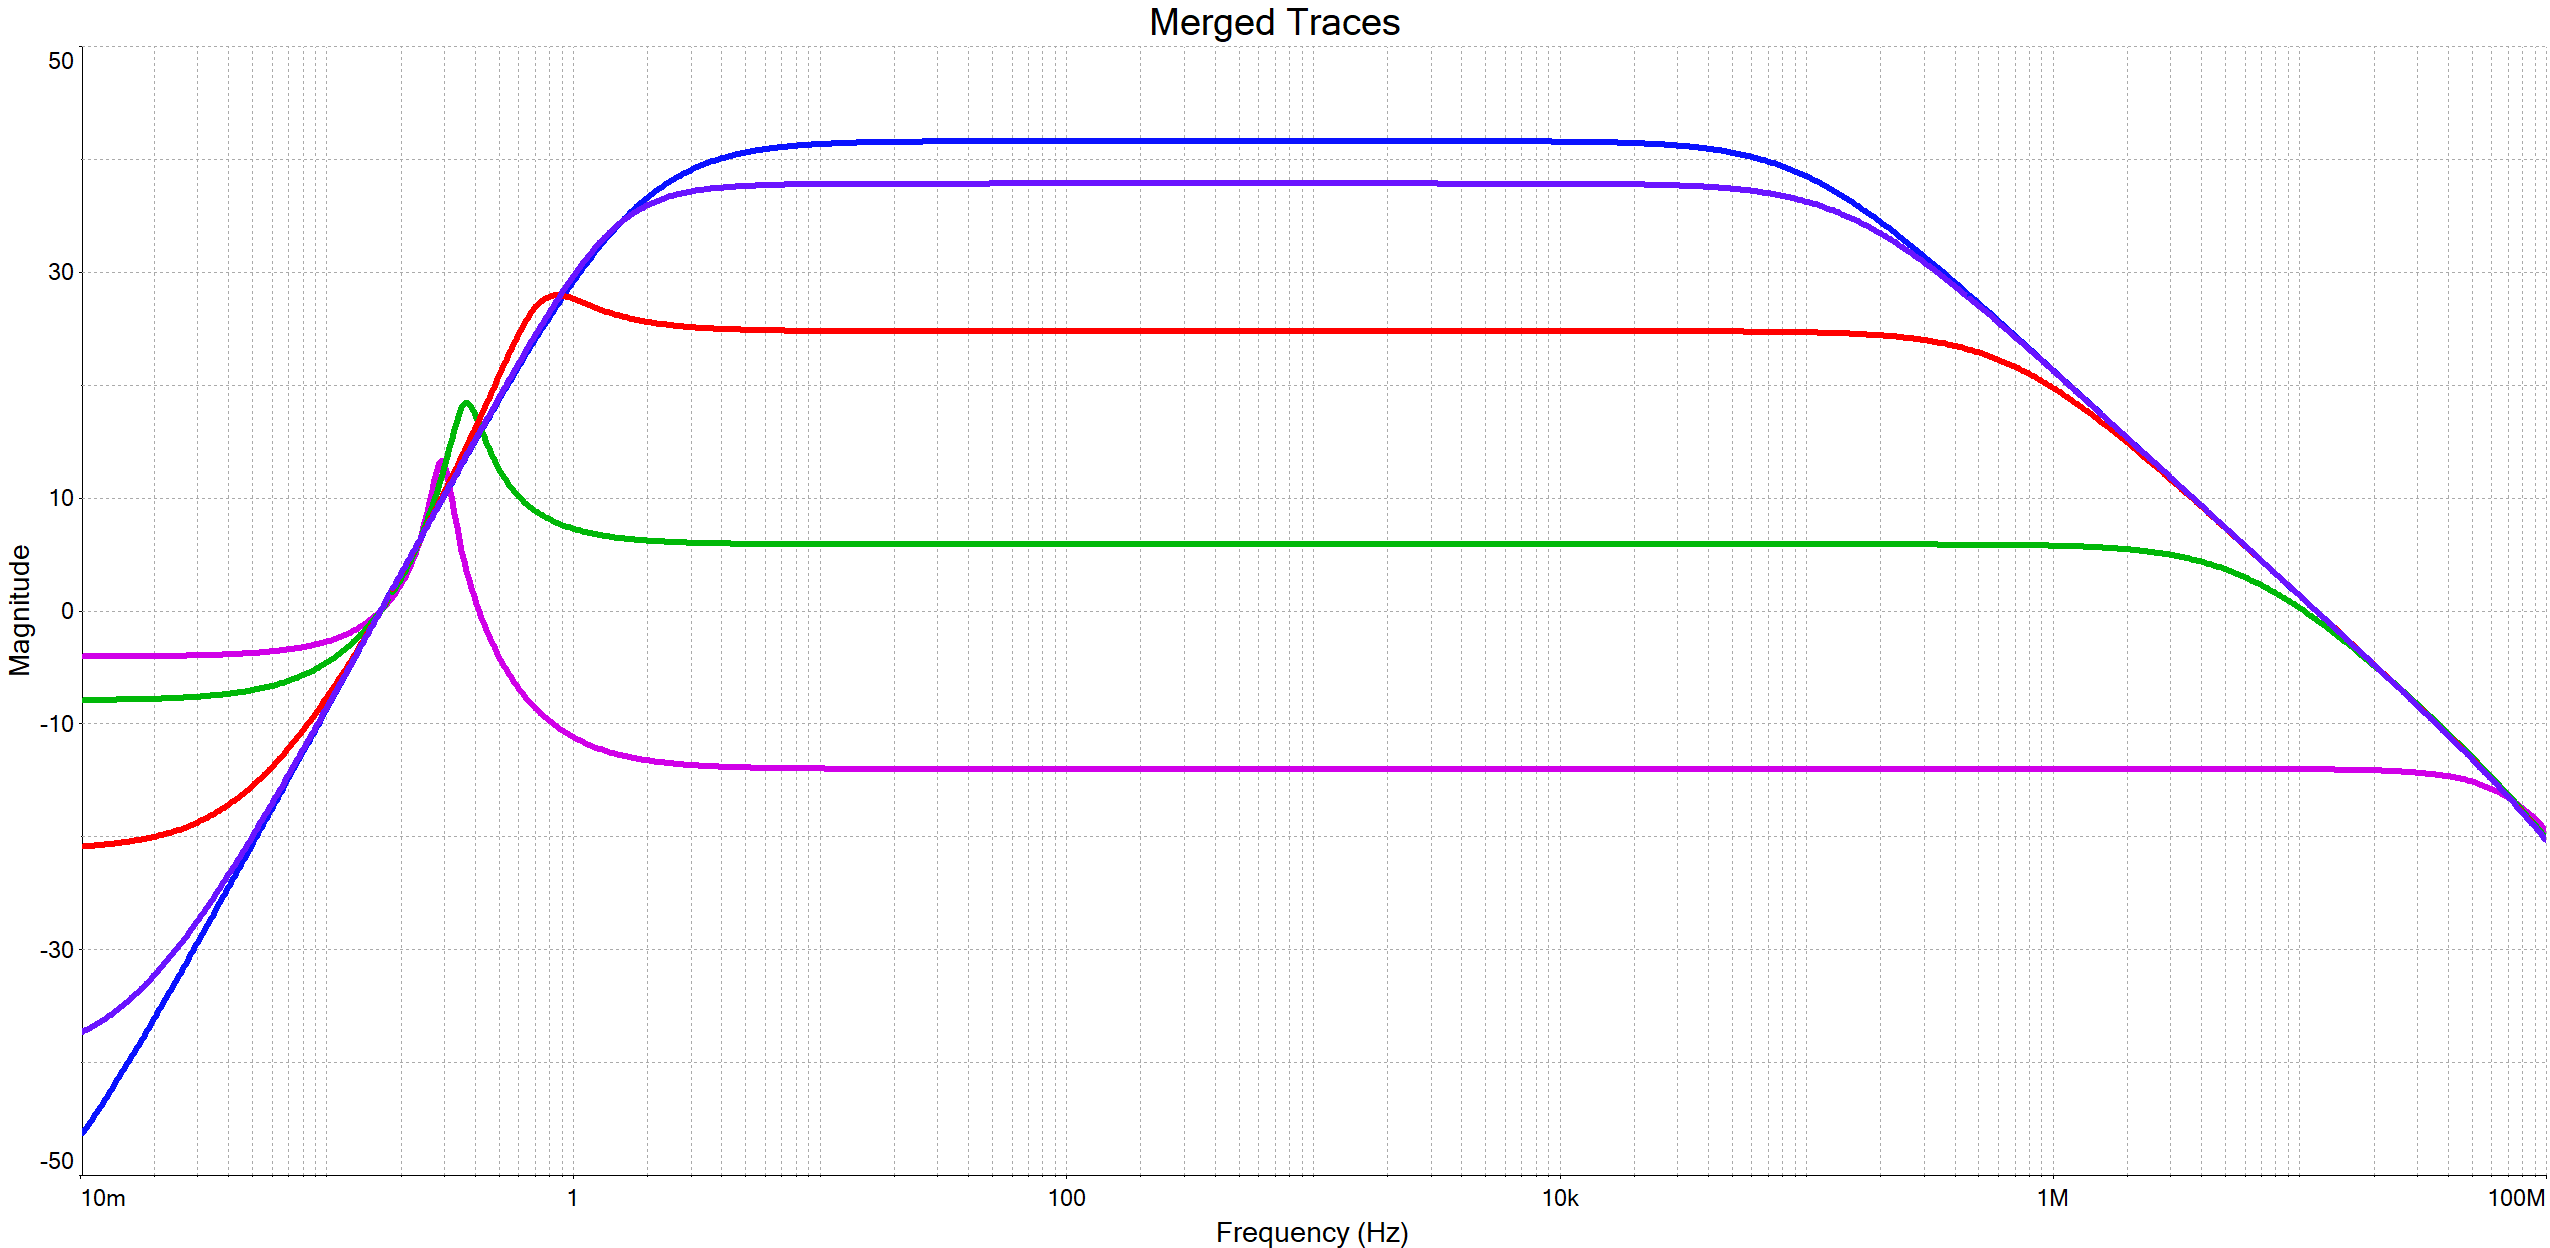
\includegraphics[height=0.45\textwidth]{Images/partcbode1k.png}\\
    \caption{Closed Loop Frequency Response with Different $R_f$ Values}
    \label{fig:clfreqresponsediffvalues}
\end{figure}
\FloatBarrier

For the calculated values, the calculations were performed the same way it was done in the 
previous part. Since we need to measure our $\beta$ value however, we can use the following
equation to use the measured values to solve for our measured $\beta$:
\begin{flalign}
&\beta_{measured}= \frac{A_f-A^{'}}{A_fA^{'}}\nonumber
\end{flalign}

Since our open loop gain is the same value as found in the previous section, we only need to measure
our $A_f$ values from the bode plot. However, once we measure the gain from the bode plot, we need
to convert it's values from $\frac{V}{V}$ to $\frac{V}{A}$. We can do this by multiplying the measured
value by $5k\Omega$, similar to the way it was converted in the previous section. Once we have
$A_f$ in $\frac{V}{V}$, we can then use that value to calculate our $\beta_{measured}$. The measured 
and calculated values are shown below:

\begin{table}[h!]
    \centering
    \begin{tabular}{lllll}
  
    $R_f(\Omega)$ & \begin{tabular}[c]{@{}l@{}}Measured  \\ $A_f(\frac{V}{A})$\end{tabular} & \begin{tabular}[c]{@{}l@{}}Measured \\ $\beta$(S)\end{tabular} & \begin{tabular}[c]{@{}l@{}}Calculated \\ $A_f(\frac{V}{A})$\end{tabular} & \begin{tabular}[c]{@{}l@{}}Calculated \\ $\beta$(S)\end{tabular} \\ \cline{1-5}
    1k & -995.5 & -1.003e-3 & -998.435 & -0.001 \\ 
    10k & -9.820k & -1.0027e-4 & -9.845k & -0.0001 \\
    100k & -86.240k & -1.0028e-5 & -86.446k & -0.00001 \\
    1M & -388.995k & -1.0028e-6 & -389.420k & -0.000001 \\
    10M & -599.425k & -1.0034e-7 & -681.2342k & -0.0000001
    \end{tabular}
    \caption{Measured and Calculated Feedback Values}
    \label{Measuredcalculatedfeedbackvalues}
\end{table}
\FloatBarrier

Comparing the calculated values and the measured values, we can see that for each value 
of $R_f$, the calculated and measured values are mostly accurate to the simulated values.
We can see that at $R_f=10M\Omega$ that the measured and calculated values are not 
as close to the simulated values. This could be due to inaccuracies in the simulation, or 
assumptions in the calculation. 

\subsubsection{Part 4}
To find the input and output resistance of the amplifier at different values of $R_f$ and 
at 1kHz, we will be using the same method as done previously to measure each of those values.
To find the calculated values of the input and output resistance for each $R_f$, we 
will be using the calculated values of $\beta$ for the corresponding $R_f$ value. We 
will be using the same formula as done previously to find the measured and calculated
values of $R_{of}$ and $R_{if}$. For the ``amount of feedback'', we will be abbreviating it on our table as ``A.o.F.''. 
To calculate it, we will be using 1+$A'\beta$. This is because this is the way that feedback is accounted for in the 
calculations for the input and output resistance calculations as shown below:
\begin{center}
$R_{of/if}=\frac{R_{in/out}}{1+A'\beta}$
\end{center}
Therfore the ``amount of feedback is calculated by the denominator of the above equation.''
The measured values are shown below:

\begin{table}[h!]
    \centering
    \begin{tabular}{lllll}
    
    $R_f (\Omega)$ & Measured  $R_{if}(\Omega)$ & Measured $R_{of}(\Omega)$ & Calculated $R_{if}(\Omega)$ & Calculated  $R_{of}(\Omega)$ \\ \cline{1-5}
    10k & 26.763 & 1.117 & 39.658 & 0.957 \\ 
    100k & 266.393 & 8.457 & 348.204 & 8.406  \\
    1M & 2.663k & 37.606 & 1.568k & 37.866 
    \end{tabular}
    \caption{Measured and Calculated $R_{of}$ and $R_{if}$ Values}
    \label{tab:measuredcalcrifrof}
\end{table}

For the estimated value, we will be using the measured values from Table \ref{tab:measuredcalcrifrof}. For the predicted 
values, we will be calculating it with the $\beta$ and $A'$ values that we already know (values from parts 2 and 3).

Below is the Amount of feedback measured and calculated values:

\begin{table}[h!]
    \centering
    \begin{tabular}{llll}
    
    $R_f(\Omega)$ & Predicted A.o.F & \begin{tabular}[c]{@{}l@{}}Measured A.o.F \\ (from $R_{if}$)\end{tabular} & \begin{tabular}[c]{@{}l@{}}Measured \\ A.o.F (from $R_{of}$)\end{tabular} \\ \cline{1-4}
    10k & 64.7786 & 95.991 & 55.521 \\ 
    100k & 7.37786 & 9.644 & 7.333 \\
    1M & 1.637786 & 0.965 & 1.649
    \end{tabular}
    \caption{Measured and Predicted ``Amount of Feedback''}
    \label{aof}
\end{table}

We can see that comparing the A.o.F. between the measured and the predicted values, they are more accurate to each other
as we increase the $R_f$ value. We can determine that because we can see that the differences between the measured and
predicted continue to decrease as $R_f$ increases. We can also observe that the A.o.F. from the output resistance is more
accurate than the value calculated from the input resistance. However, the observation that each value of A.o.F. continues
to be more accurate as $R_f$ increases is still accurate to both methods of calculating A.o.F.. This could happen due to 
assumptions in the calculation that is not accounted for compared to the simulation.  

We can also see from table \ref{tab:measuredcalcrifrof}  that the measured and calculated values of $R_{of}$ 
are very accurate to the measured value. However, we can see that the input impedance
calculations are not as accurate to the measured values. This could also be due to 
inaccuracies in the simulation, or assumptions in the calculation.

\subsubsection{Part 5}

From the class notes[1], we find that the de-sensitivity factor is found by 1+$A\beta$. If $R_f = \infty$,
then, our de-sensitivity factor is 1 since the $A\beta$ portion equates to 0 because in this case, $\beta=\frac
{1}{\infty}$.
Simulating for $R_f=\infty$, we find:

\begin{table}[h!]
    \centering
    \begin{tabular}{ll}
    $R_f(\Omega)$ & Measured Gain($\frac{V}{V}$) \\ \hline
    9.9k & -126.848 \\ 
    10k & -127.553 \\
    10.1k & -128.201
    \end{tabular}
    \caption{Measured Output with $R_f=\infty$}
    \label{measuredoutinf}
\end{table}
\FloatBarrier

Simulating for $R_f=100k\Omega$, we find:

\begin{table}[h!]
    \centering
    \begin{tabular}{ll}
    $R_f(\Omega)$ & Measured Gain($\frac{V}{V}$) \\ \hline
    9.9k & -17.235 \\ 
    10k & -17.248 \\
    10.1k & -17.260
    \end{tabular}
    \caption{Measured Output with $R_f=100k\Omega$}
    \label{measuredout}
\end{table}
\FloatBarrier 

With these values, we can find the de-sensitivity factor for $R_f=100k\Omega$. The values of the 
gain does not change much for the different values of $R_c$. The de-sensitivity factor is found to be:

\begin{table}[h!]
    \centering
    \begin{tabular}{ll}
    $R_f(\Omega)$ & De-Sensitivity Factor \\ \hline
    9.9k & 7.3424 \\ 
    10k & 7.378 \\
    10.1k & 7.410
    \end{tabular}
    \caption{De-Sensitivity Factor}
    \label{desens}
\end{table}
\FloatBarrier

Comparing the gain values from parts 2 and 3, we 
find that the gain values are very similar to each other. Therefore, we find that this 
circuit is desensitized. For smaller values of $R_f$, an observation can be made that the gain is larger at mid band.
This could occour because the de-sensitivity factor decreases with a smaller $R_f$ value. With the lower de-sensitivity 
factor, the mid band gain would then be larger; compared to the gain from a larger $R_f$ value. 

\newpage
\section{Appendix}

\begin{flalign}
    &k = 3 - \sqrt{2} = 1+\frac{R_2}{R_1}\\
    &A_m = 1+\frac{R_2}{R_1}\\
    &R_2+R_1=10k\Omega\\
    &R_1 = \frac{10000}{-\sqrt{2}+3}\Omega\\
    &R_2 = \frac{1}{7}(-10000\sqrt{2}+40000)\Omega
\end{flalign}
\section{References}
1. ELEC 301 Class notes 
\newline
2. Mini Project 4 Document
\newline
3. Standard Resistor and Capacitor Values (Canvas)
\newline
4. Circuit Maker SPICE Model
\newline
5. Sedra, Smith - Microelectronic Circuits 5th Edition

\end{document}